\section{Estimate the Steering Matrix}
Estimation of $\ma{A}$ without knowledge of $\ma{S}$:\\
$\ma{X}=\ma{A}\ma{S}+\ma{\nu}$\\
To determine \ma{A} we could use pilots like we did already earlier in this lecture. But here we want to derive a method that works without sending known symbols over the channel. This is called "Blind Channel Estimation".\\ \\
\underline{Non-linear estimation for \ma{A}:}\\
\begin{doublespace}
$\ma{A}=\mat{\vec{a}[\Theta_1]&\vec{a}[\Theta_2]&\shdots&\vec{a}[\Theta_d]} \in\mathbb{C}^{M\times d}$\\
\begin{figure}[H]
	\centering
		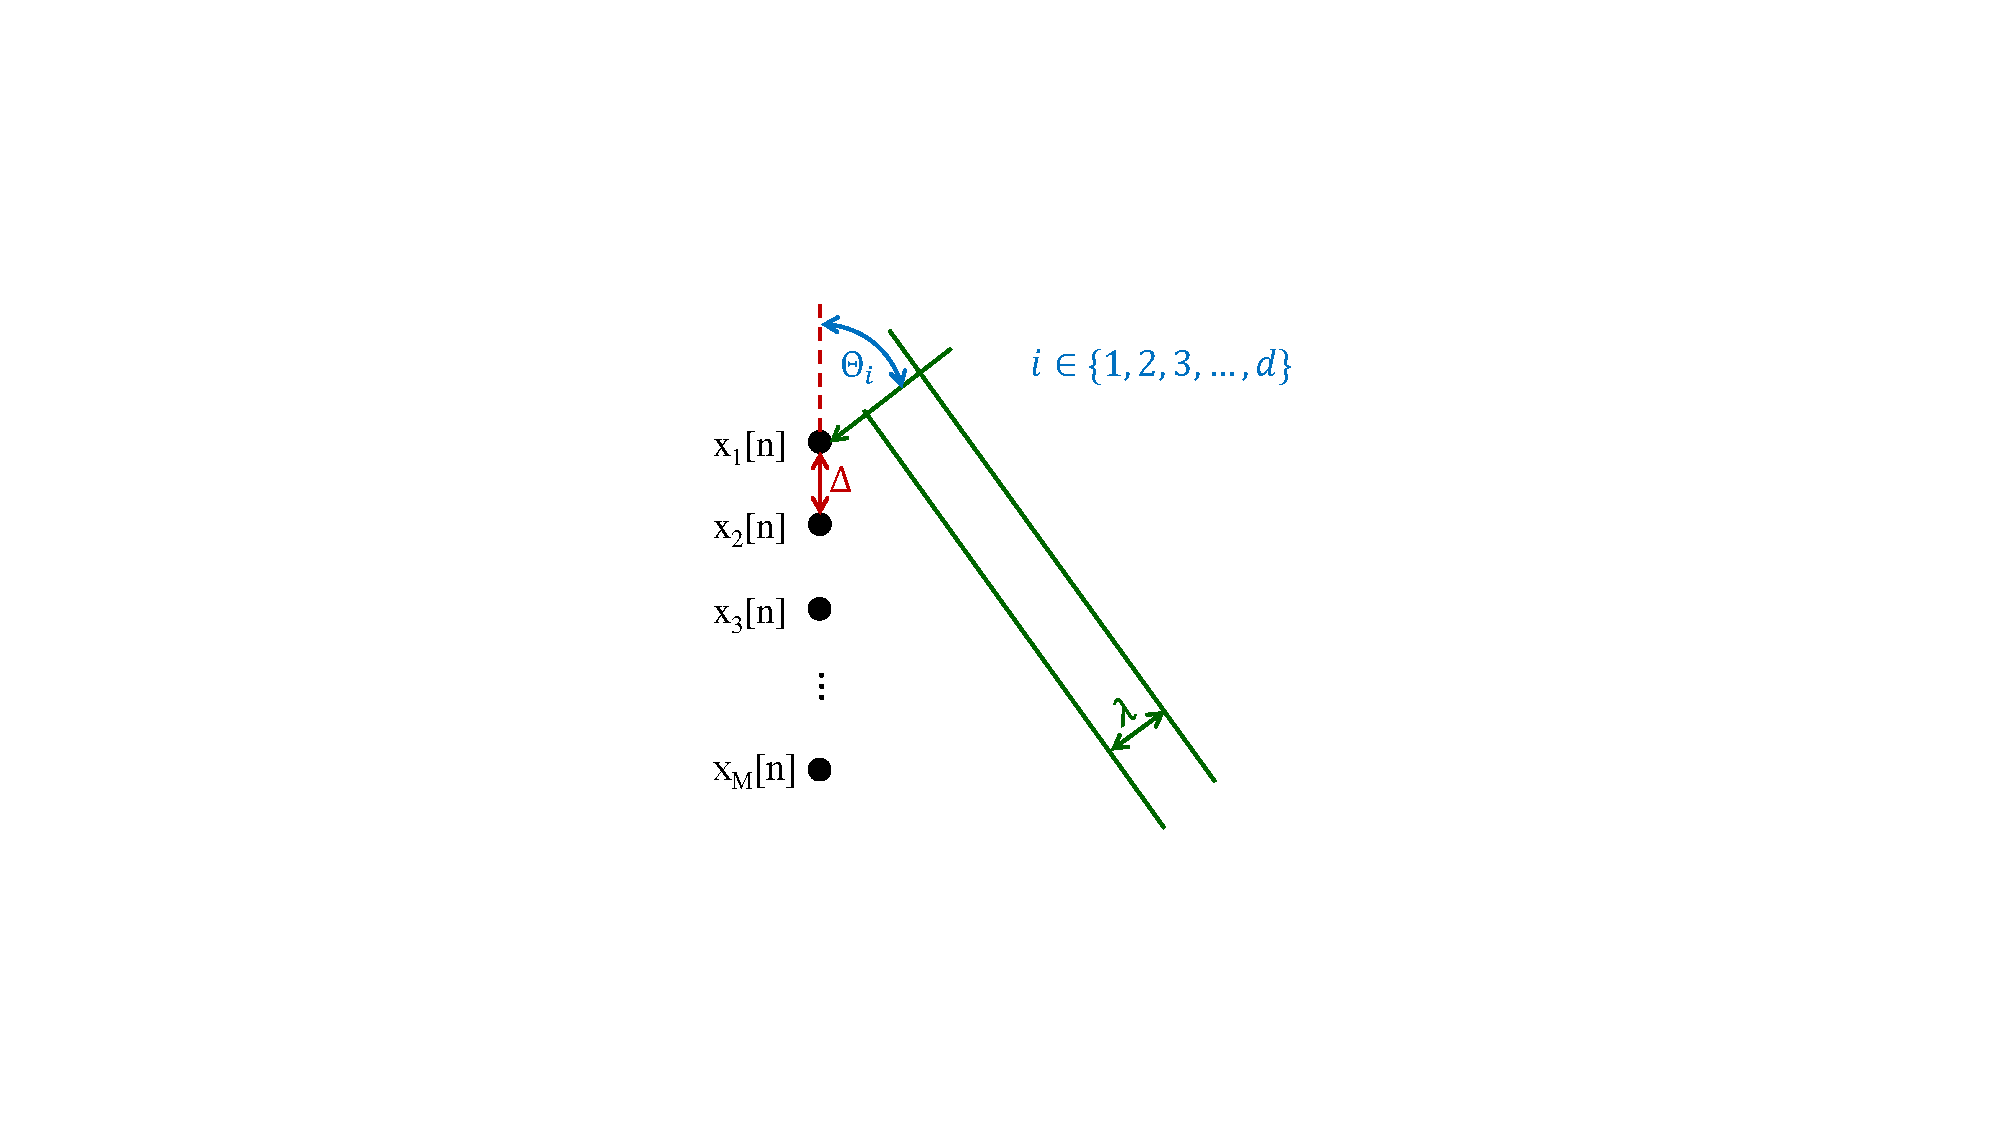
\includegraphics[trim =6cm 5.5cm 6cm 4cm, clip, width=0.70\textwidth]{graphics/ULA_Angle_theta_M_Sensors.pdf}
	\caption{Unform Linear Array (ULA) with $M$ sensors}
	\label{fig:ULA_Angle_theta_M_Sensors}
\end{figure}

$\vec{a}(\Theta_i)=\mat{1\\e^{-\j2\pi\frac{\Delta}{\lambda}\cos(\Theta_i)}\\e^{-2\j2\pi\frac{\Delta}{\lambda}\cos(\Theta_i)}\\e^{-3\j2\pi\frac{\Delta}{\lambda}\cos(\Theta_i)}\\\shdots\\e^{-(M-1)\j2\pi\frac{\Delta}{\lambda}\cos(\Theta_i)}}  $ \\ \\
\mybox{
$\mu:=2\pi\frac{\Delta}{\lambda}\cos(\Theta)\qquad \mu_i:=2\pi\frac{\Delta}{\lambda}\cos(\Theta_i)$\qquad $\mu$ is the phase of the signal.
}\\ \\
$\vec{a}(\mu_i)=\mat{1\\e^{-\j\mu_i}\\e^{-2\j\mu_i}\\e^{-3\j\mu_i}\\\svdots\\\\e^{-(M-1)\j\mu_i}}=\mat{1\\\xi^1\\\xi^2\\\xi^3\\\svdots\\\xi^{M-1}}$ "Vandermonde vector"\\ \\
$\Theta=\arccos\left(\frac{\mu}{2\pi\frac{\Delta}{\lambda}}\right)$\\
$\vec{a}(\mu)=\vec{a}(\mu+2\pi n); \quad n\in\{0,\pm1,\pm2,\ldots\}$\\
\mybox{
What is now the corresponding angle? $\Theta$ or $\Theta'$?\\
$\mu+2\pi n = 2\pi\frac{\Delta}{\lambda}\cos(\Theta')$\\
$\mu=2\pi\frac{\Delta}{\lambda}\cos(\Theta)$
}\\
$2\pi\frac{\Delta}{\lambda}\cos(\Theta)+2\pi n = 2\pi\frac{\Delta}{\lambda}\cos(\Theta')$\\
$\cos(\Theta)+\frac{2\pi n}{2\pi\frac{\Delta}{\lambda}}=\cos(\Theta')$\\
$\Theta'=\arccos\underbrace{\left(\frac{n}{\frac{\Delta}{\lambda}}+\cos(\Theta)\right)}_{\Phi};\quad n\in\{0,\pm1,\pm2,\ldots\}$\\
if $\frac{\Delta}{\lambda} < \frac{1}{2}$ \Ra $n=0$ only possible for existing values $\Theta=\Theta'$\\ \\
if $\frac{\Delta}{\lambda}=\frac{1}{2} \Ra (\Theta,\Theta')\in\{(0,\pi),(\pi,0)\}$\\
Determine the error of $\Theta$ with respect to $\mu$:\\
$\Theta=\arccos\left(\frac{\mu}{2\pi\frac{\Delta}{\lambda}}\right)$\\
$\frac{\partial \Theta}{\partial \mu}=\frac{1}{\Delta/\lambda}\cdot \frac{1}{\sqrt{4\pi^2-\left(\frac{\mu}{\Delta/\lambda}\right)^2}}$\\
$\min\limits_\mu\frac{\partial \Theta}{\partial \mu}=\frac{\partial \Theta}{\partial \mu}\left.\right|_{\mu=0}=\frac{1}{2\pi \frac{\Delta}{\lambda}}$\\
Estimate $\mu$ with error $e_{\mu}=\pm\Delta\mu$\\
Then $\Theta$ with error $e_{\Theta}\approx\frac{\partial \Theta}{\partial \mu}\Delta\mu=\frac{1}{\Delta/\lambda}\cdot \frac{1}{\sqrt{4\pi^2-\left(\frac{\mu}{\Delta/\lambda}\right)^2}}\Delta\mu$\\
Note that the function for $\frac{\partial \Theta}{\partial \mu}$ has a pole:\\
$4\pi^2=\frac{\mu^2}{(\frac{\Delta}{\lambda})^2}; \qquad 4\pi^2(\frac{\Delta}{\lambda})^2=\mu^2 \Rightarrow \mu=2\pi \frac{\Delta}{\lambda}$\\
$\frac{\partial \Theta}{\partial \mu}\left.\right|_{\mu=2\pi \frac{\Delta}{\lambda}} = \infty$\\
if $\frac{\Delta}{\lambda} = \frac{1}{2} \Rightarrow \mu=\pi$ is worst for estimating $\Theta$
\Ra in practice we can therefore allow $\frac{\Delta}{\lambda}=\frac{1}{2}$ because the situition is anyway very bad for estimating $\Theta$.\\ \\
$\frac{\partial \Theta}{\partial \mu} \leq 2 \min \frac{\partial \Theta}{\partial \mu}$\\

\begin{figure}[H]
	\centering
		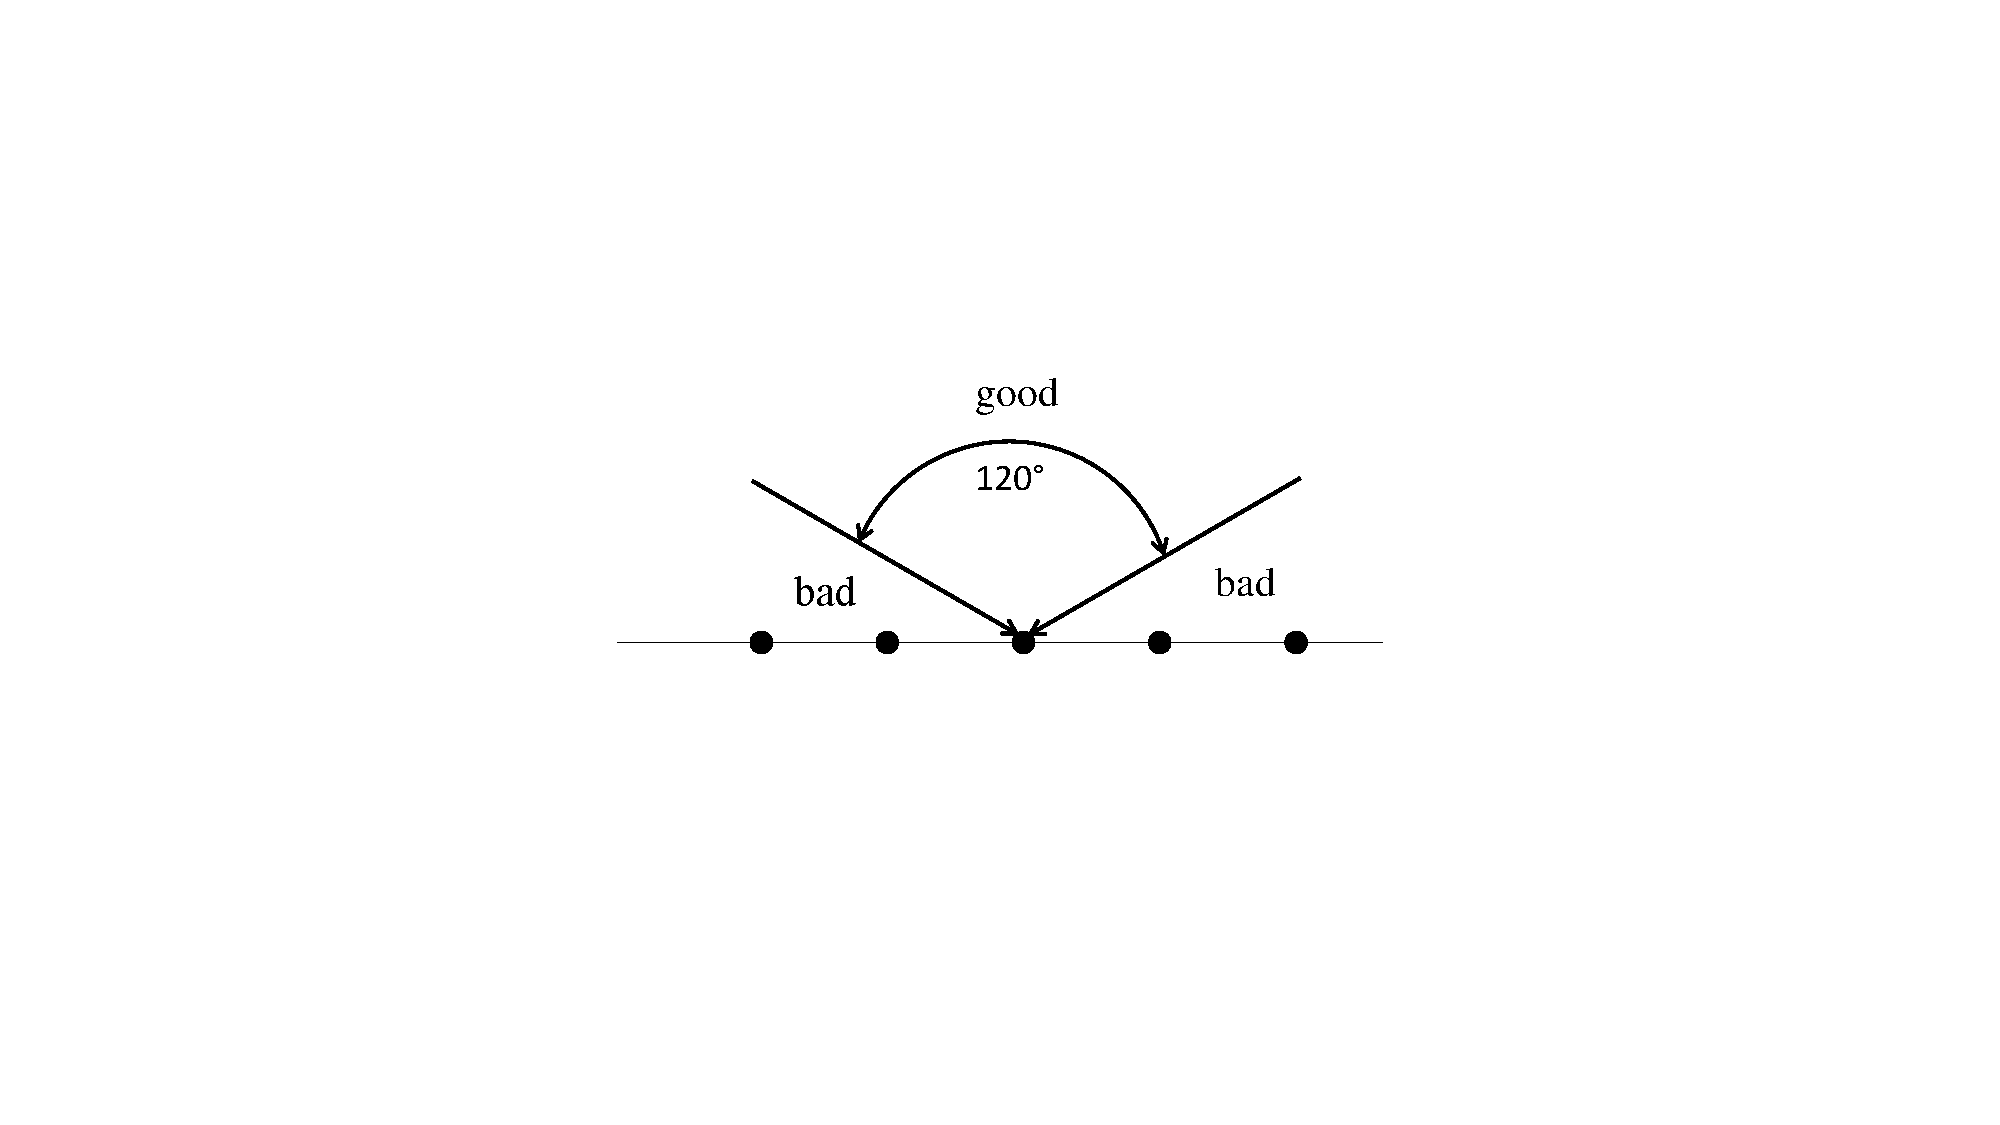
\includegraphics[trim =8cm 8cm 8cm 6cm, clip, width=0.70\textwidth]{graphics/Behaviour_of_estimation_of_mu_for_regions.pdf}
	\caption{Behaviour of the estimated $\mu$ for different angles }
	\label{fig:Behaviour_of_estimation_of_mu_for_regions}
\end{figure}

\begin{tabular}{rl}
d: & Number of arriving wavefronts\\
 & unknown to the receiver\\
 & needs to be estimated\\
$\Theta_1,\,\Theta_2,\ldots\Theta_d$:& Directions of arrival (DoA)\\
\end{tabular}\\
$\mu_i=2\pi \frac{\Delta}{\lambda}\cos(\Theta_i)$\\
\textbf{From now on we choose} $\frac{\Delta}{\lambda}=\frac{1}{2}$\\
Then:\\
\mybox{
$\mu_i=\pi\cos(\Theta_i)$
}
\begin{figure}[H]
	\centering
		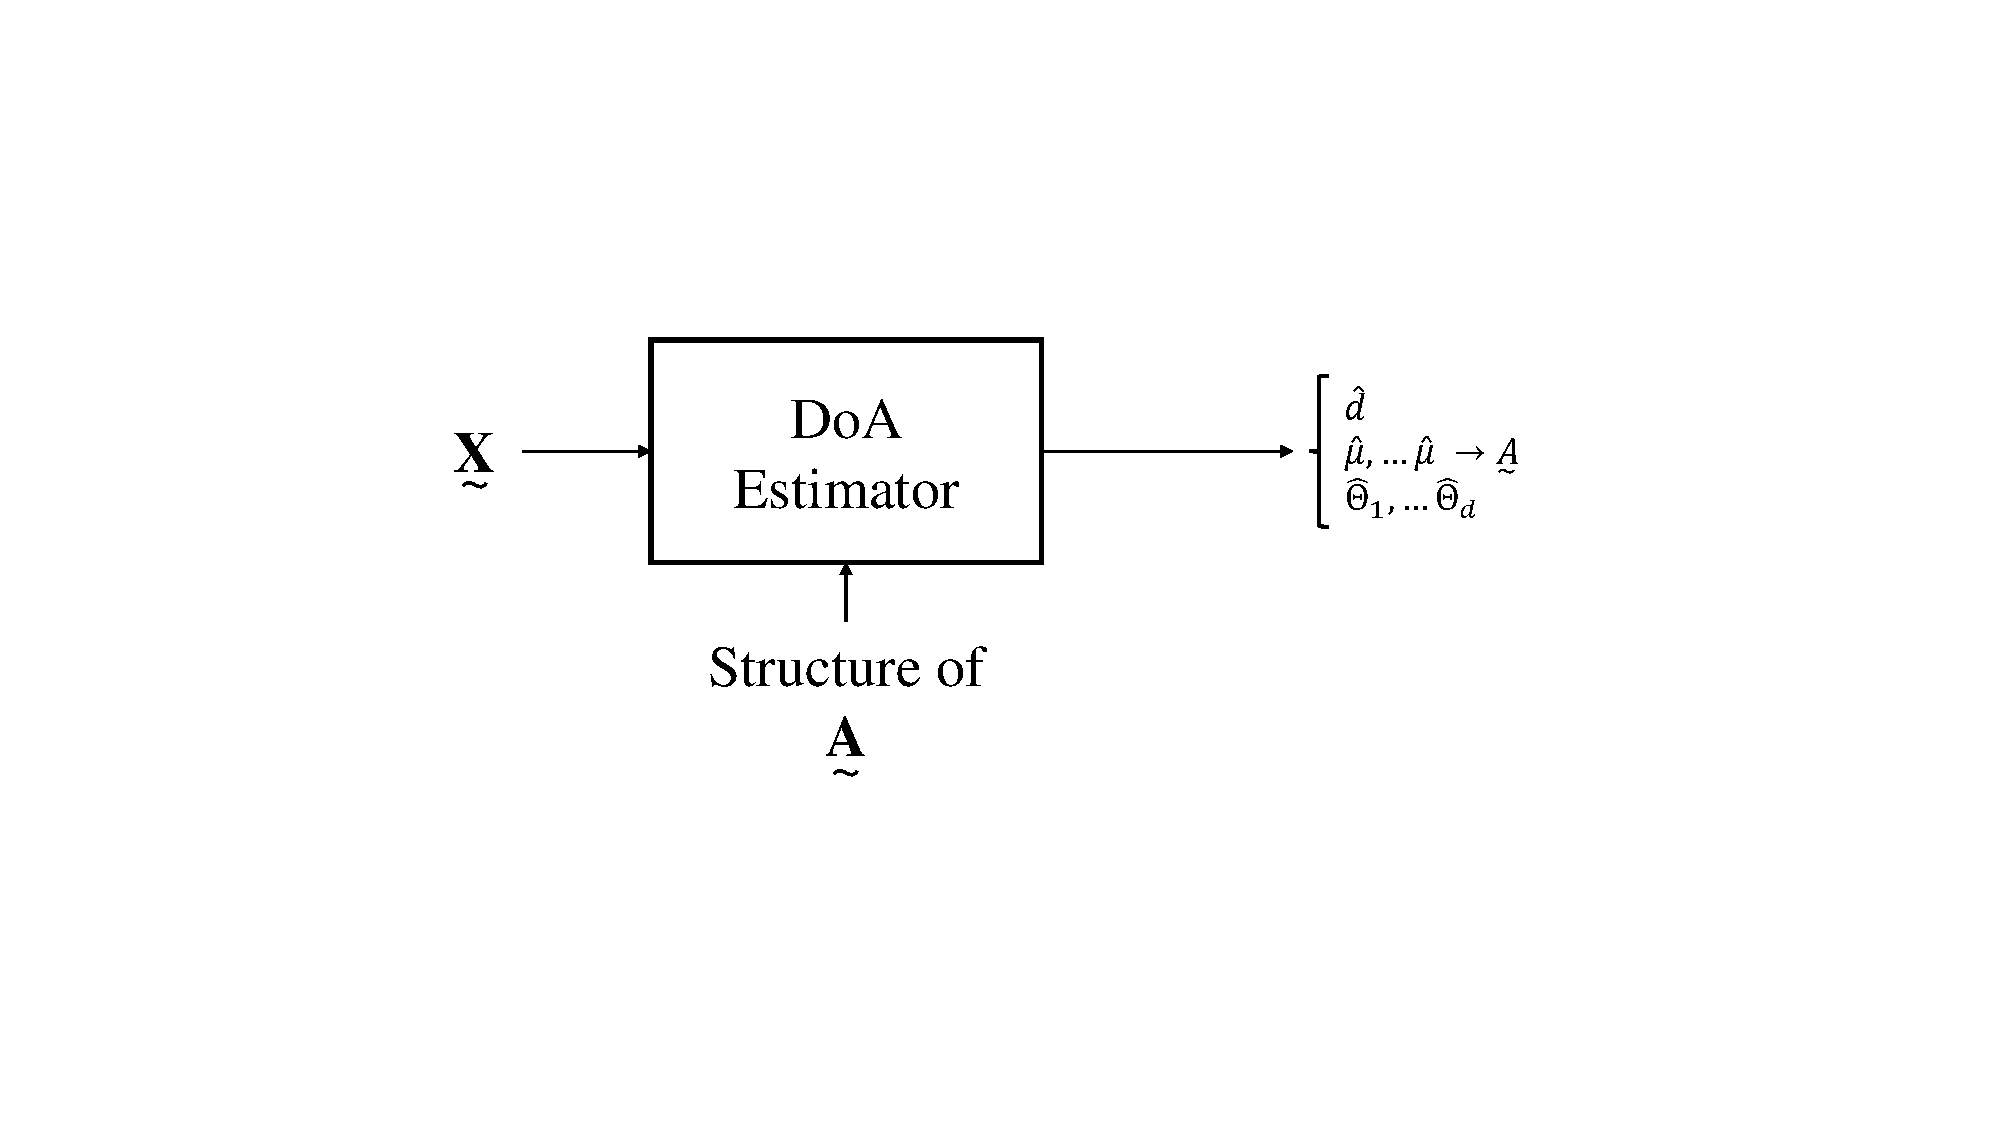
\includegraphics[trim =4cm 5.5cm 4cm 4cm, clip,width=0.70\textwidth]{graphics/Block_diagram_DoA_estimator.pdf}
	\caption{Simple block diagram of a DoA (Dimension of Arrival) Estimator}
	\label{fig:Block_diagram_DoA_estimator}
\end{figure}
\end{doublespace}

\subsection{Space-Discrete Fourier Transform}
\begin{figure}[H]
	\centering
		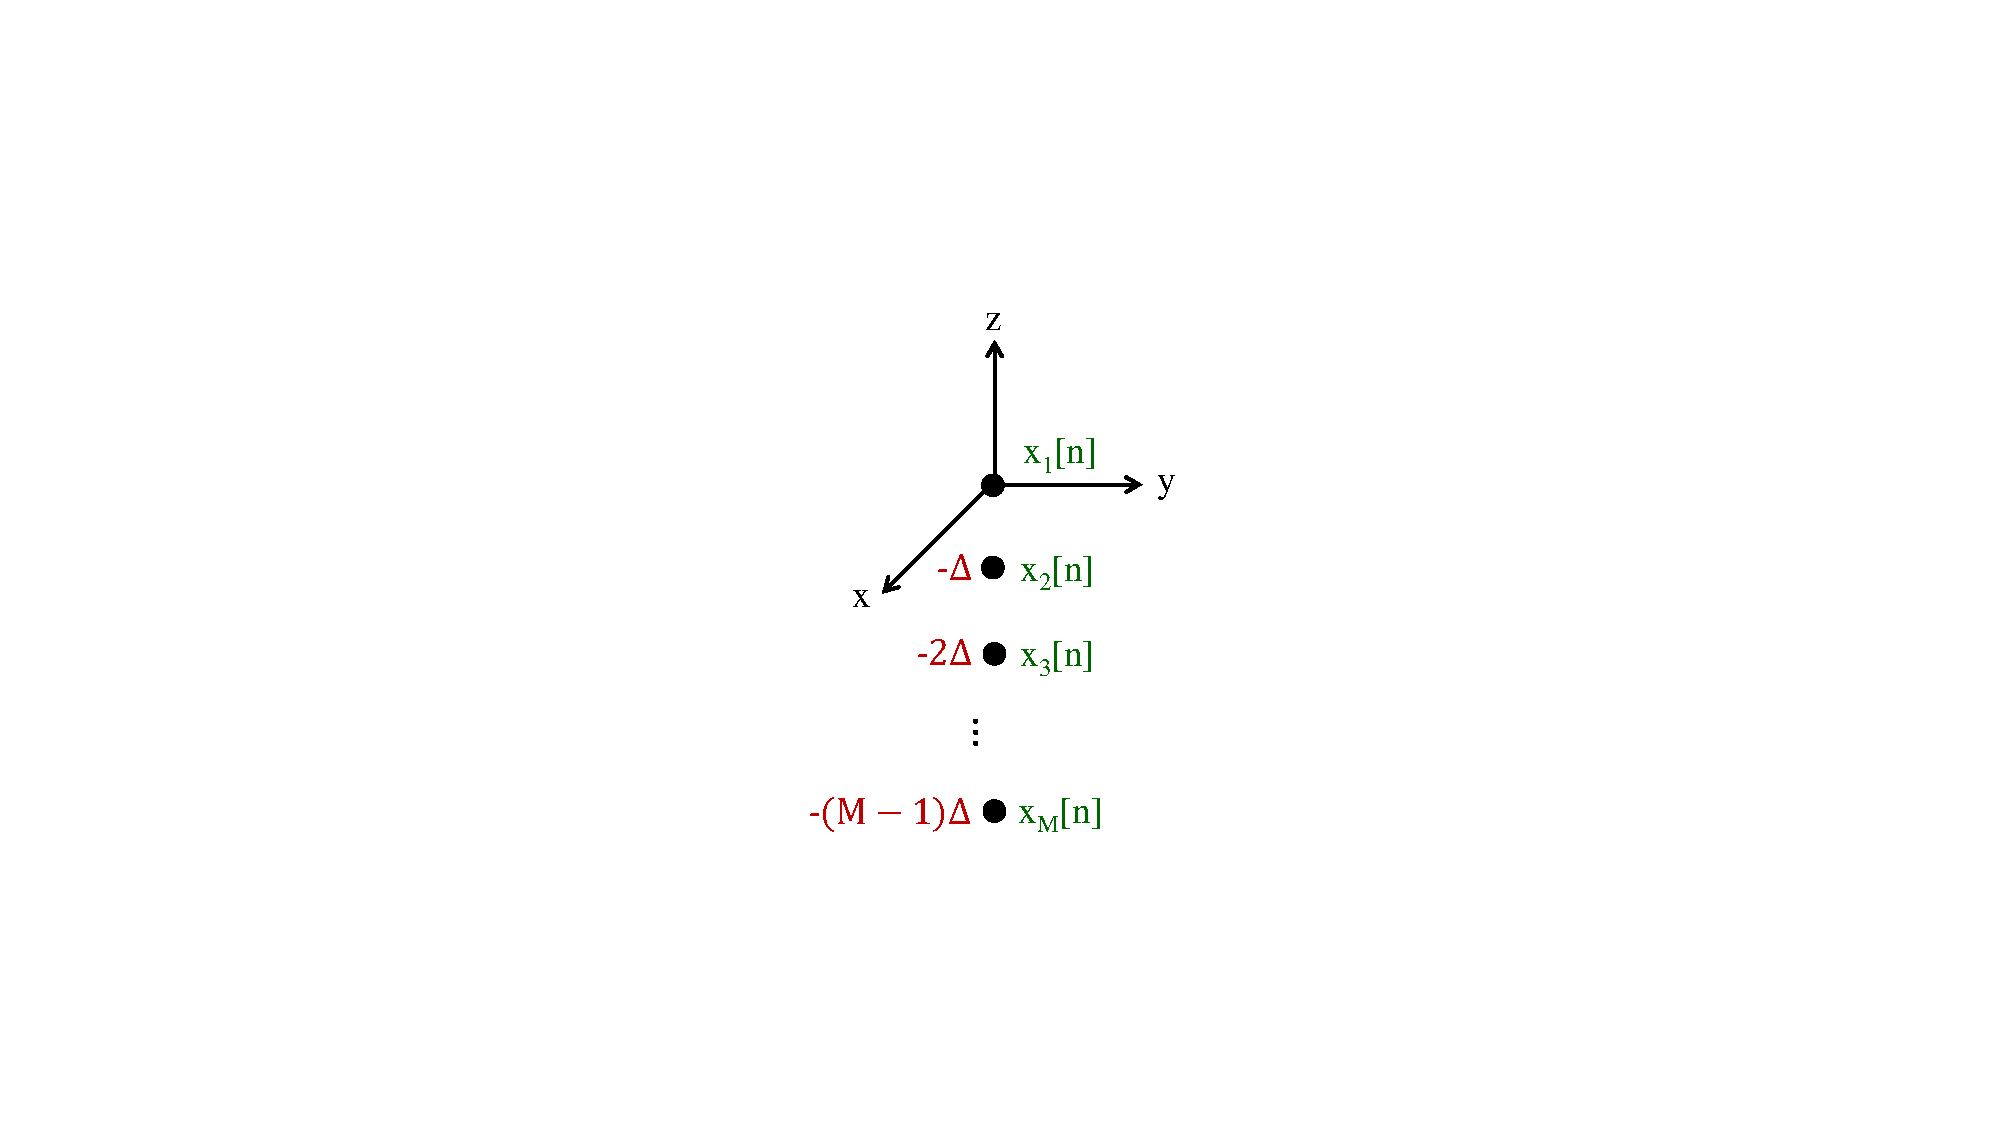
\includegraphics[trim =6cm 4.5cm 6cm 4cm, clip, width=0.70\textwidth]{graphics/ULA_space-discrete_fourier_transform.pdf}
	\caption{Sensor arrangement for the Space-Discrete Fourier Transform}
	\label{fig:ULA_space-discrete_fourier_transform}
\end{figure}


\begin{itemize}
	\item sampling in space: $x_k[n]=g(z)\left.\right|_{z=-(k-1)\Delta}$ \pfeil $g(z)= field$
	\item Space Fourier Transform: $G(\tilde{f})=\int\limits_{-\infty}^{\infty}{g(z)e^{-\j2\pi\tilde{f}z}dz}$
\end{itemize}
The "Space Fourier Transform" is related to the Time Fourier Transform, just replace time by space ($t$ by $z$) and the frequency $f$ by the space frequency $\tilde{f}$.\\
$\tilde{f}$: space-frequency $\qquad [\tilde{f}]=\frac{1}{m}=m^{-1}$\\
\Ra Problem: g(z) is not known to us everywhere. We just know it at some discrete points. Therefor we sample it:\\
$h(z)=g(z)\sum\limits_{k=0}^{M-1}{\delta(z+\Delta k)}$\\
\rule{\textwidth}{0.4pt}
\textbf{Recall:}\\
$\delta(z)=0, \forall z \neq 0$\\
$\int\limits_{-\infty}^{\infty}{\delta(z)dz}=1$\\
\rule{\textwidth}{0.4pt}
\begin{flalign*}
H(\tilde{f})&=\int\limits_{-\infty}^{\infty}{h(z)e^{-\j2\pi\tilde{f}z}dz}&&\\
&=\int\limits_{-\infty}^{\infty}{g(z)\left(\sum\limits_{k=0}^{M-1}{\delta(z+\Delta k)}\right)e^{-\j2\pi\tilde{f}z}dz}&&\\
&=\sum\limits_{k=0}^{M-1}{\int\limits_{-\infty}^{\infty}{g(z)\delta(z+\Delta k)e^{-\j2\pi\tilde{f}z}dz}}&&\\
&=\sum\limits_{k=0}^{M-1}{\int\limits_{-\infty}^{\infty}{g(-\Delta k)\delta(z+\Delta k)e^{+\j2\pi\tilde{f}\Delta k}dz}}&&\\
&=\sum\limits_{k=0}^{M-1}{g(-\Delta k)e^{+\j2\pi\tilde{f}\Delta k}}\underbrace{\int\limits_{-\infty}^{\infty}{\delta(z+\Delta k)dz}}_{=1}&&\\
&=\sum\limits_{k=0}^{M-1}{\underbrace{g(-\Delta k)}_{x_{k+1}[n]}e^{+\j2\pi\tilde{f}\Delta k}dz}
\end{flalign*}
For convenience we define $\mu:=2\pi\tilde{f}\Delta$.\\
\mybox{
$H(\tilde{f})=\sum\limits_{k=0}^{M-1}{x_{k+1}[n]e^{\j\mu k}}$
}\\
$\mu$: Normalized space angular frequency (dimensionless)
Compare:\\ $\underbrace{2\pi f }_{\omega}T=\omega T = \Omega$\qquad
$2\pi\tilde{f}\Delta = \mu$ \\ \\
Recall the steering vector $\vec{a}(\mu)$ and the received signal vector $\vec{x}[n]$:\\
$\vec{a}(\mu)=\mat{1\\e^{-\j\mu}\\e^{-2\j\mu}\\e^{-3\j\mu}\\\svdots\\\\e^{-(M-1)\j\mu}}; \qquad \vec{x}[n]=\mat{\\x_2[n]\\x_3[n]\\x_4[n]\\\svdots\\x_M[n]}$\\

\mybox{
$H(\mu)=\vec{a}^H(\mu)\vec{x}[n]$\\
Note: $H(\mu)$ is just an other notation of $H(\tilde{f})$
}

\paragraph{Fourier Periodogram}
\begin{flalign*}
S(\mu):&=\frac{1}{N}\sum\limits_{n=1}^{N}{\left|\vec{a}^H(\mu)\vec{x}[n]\right|^2}=\bar{\abs{H(\mu)}^2}&&\\
&=\frac{1}{N}\sum\limits_{n=1}^{N}{\vec{a}^H(\mu)\vec{x}[n]\vec{x}^H[n]\vec{a}(\mu)}&&\\
&=\vec{a}^H(\mu)\underbrace{\left(\sum\limits_{n=1}^{N}{\vec{x}[n]\vec{x}^H[n]}\right)}_{\ma{\hat{R}}_x=\frac{1}{N}\ma{X}\ma{X}^H}\vec{a}(\mu)
\end{flalign*}
\mybox{
$S(\mu)=\vec{a}^H(\mu)\ma{\hat{R}}_x\vec{a}(\mu)\qquad \mu=2\pi\frac{\Delta}{\lambda}\cos(\Theta)$
}
Search peaks in the periodogram to find $\mu$ of incoming wave fronts.
\\ \ \\
\textbf{Example:}\\
$d=1$ (only one arriving wavefront)\\
no noise, continuous wave $s[n]=\const=1$\\
$\vec{x}[n]=\vec{a}(\mu_1)s[n]=\vec{a}(\mu_1); \qquad \mu_1=2\pi\frac{\Delta}{\lambda}\cos(\Theta_1)$ \quad find: $\Theta_1$\\
$\ma{\hat{R}}_x = \frac{1}{N}\sum\limits_{n=1}^{N}{\vec{a}(\mu_1)\vec{a}^H(\mu_1)} = \vec{a}(\mu_1)\vec{a}^H(\mu_1)$\\
\begin{flalign*}
S(\mu)&=\vec{a}^H(\mu)\ma{\hat{R}}_x\vec{a}(\mu)&&\\
&=\vec{a}^H(\mu)\vec{a}(\mu_1)\vec{a}^H(\mu_1)\vec{a}(\mu)&&\\
&=\left|\vec{a}^H(\mu)\vec{a}(\mu_1)\right|^2&&\\
&=\left|\sum\limits_{k=0}^{M-1}{e^{\j(\mu-\mu_1)k}}\right|^2
\end{flalign*}
\rule{\textwidth}{0.4pt}
\textbf{Recall:}\\
$s=1+q+q^2+\ldots+q^{M-1}$\\
$sq=q+q^2+\ldots+q^{M-1}+q^M$\\
$sq-s=q^M-1 \Rightarrow s=\frac{q^M-1}{q-1}$ (geometric series)\\
$q=e^{\j(\mu-\mu_1)}$\\
\rule{\textwidth}{0.4pt}

\begin{flalign*}
S(\mu)&=\left|\frac{e^{\j(\mu-\mu_1)M}-1}{e^{\j(\mu-\mu_1)}-1}\right|^2&&\\
&=\left|\frac{e^{\j(\mu-\mu_1)\frac{M}{2}}\cdot\left(e^{\j(\mu-\mu_1)\frac{M}{2}}-e^{-\j(\mu-\mu_1)\frac{M}{2}}\right)}{e^{\j\frac{(\mu-\mu_1)}{2}}\cdot\left(e^{\j\frac{(\mu-\mu_1)}{2}}-e^{-\j\frac{(\mu-\mu_1)}{2}}\right)}\right|^2&&\\
&=\left(\frac{\sin\left(\frac{M}{2}(\mu-\mu_1)\right)}{\sin\left(\frac{1}{2}(\mu-\mu_1)\right)}\right)^2
\end{flalign*}
$\lim\limits_{\mu\rightarrow\mu_1}S(\mu)=M^2$\\

\begin{figure}[H]
	\centering
		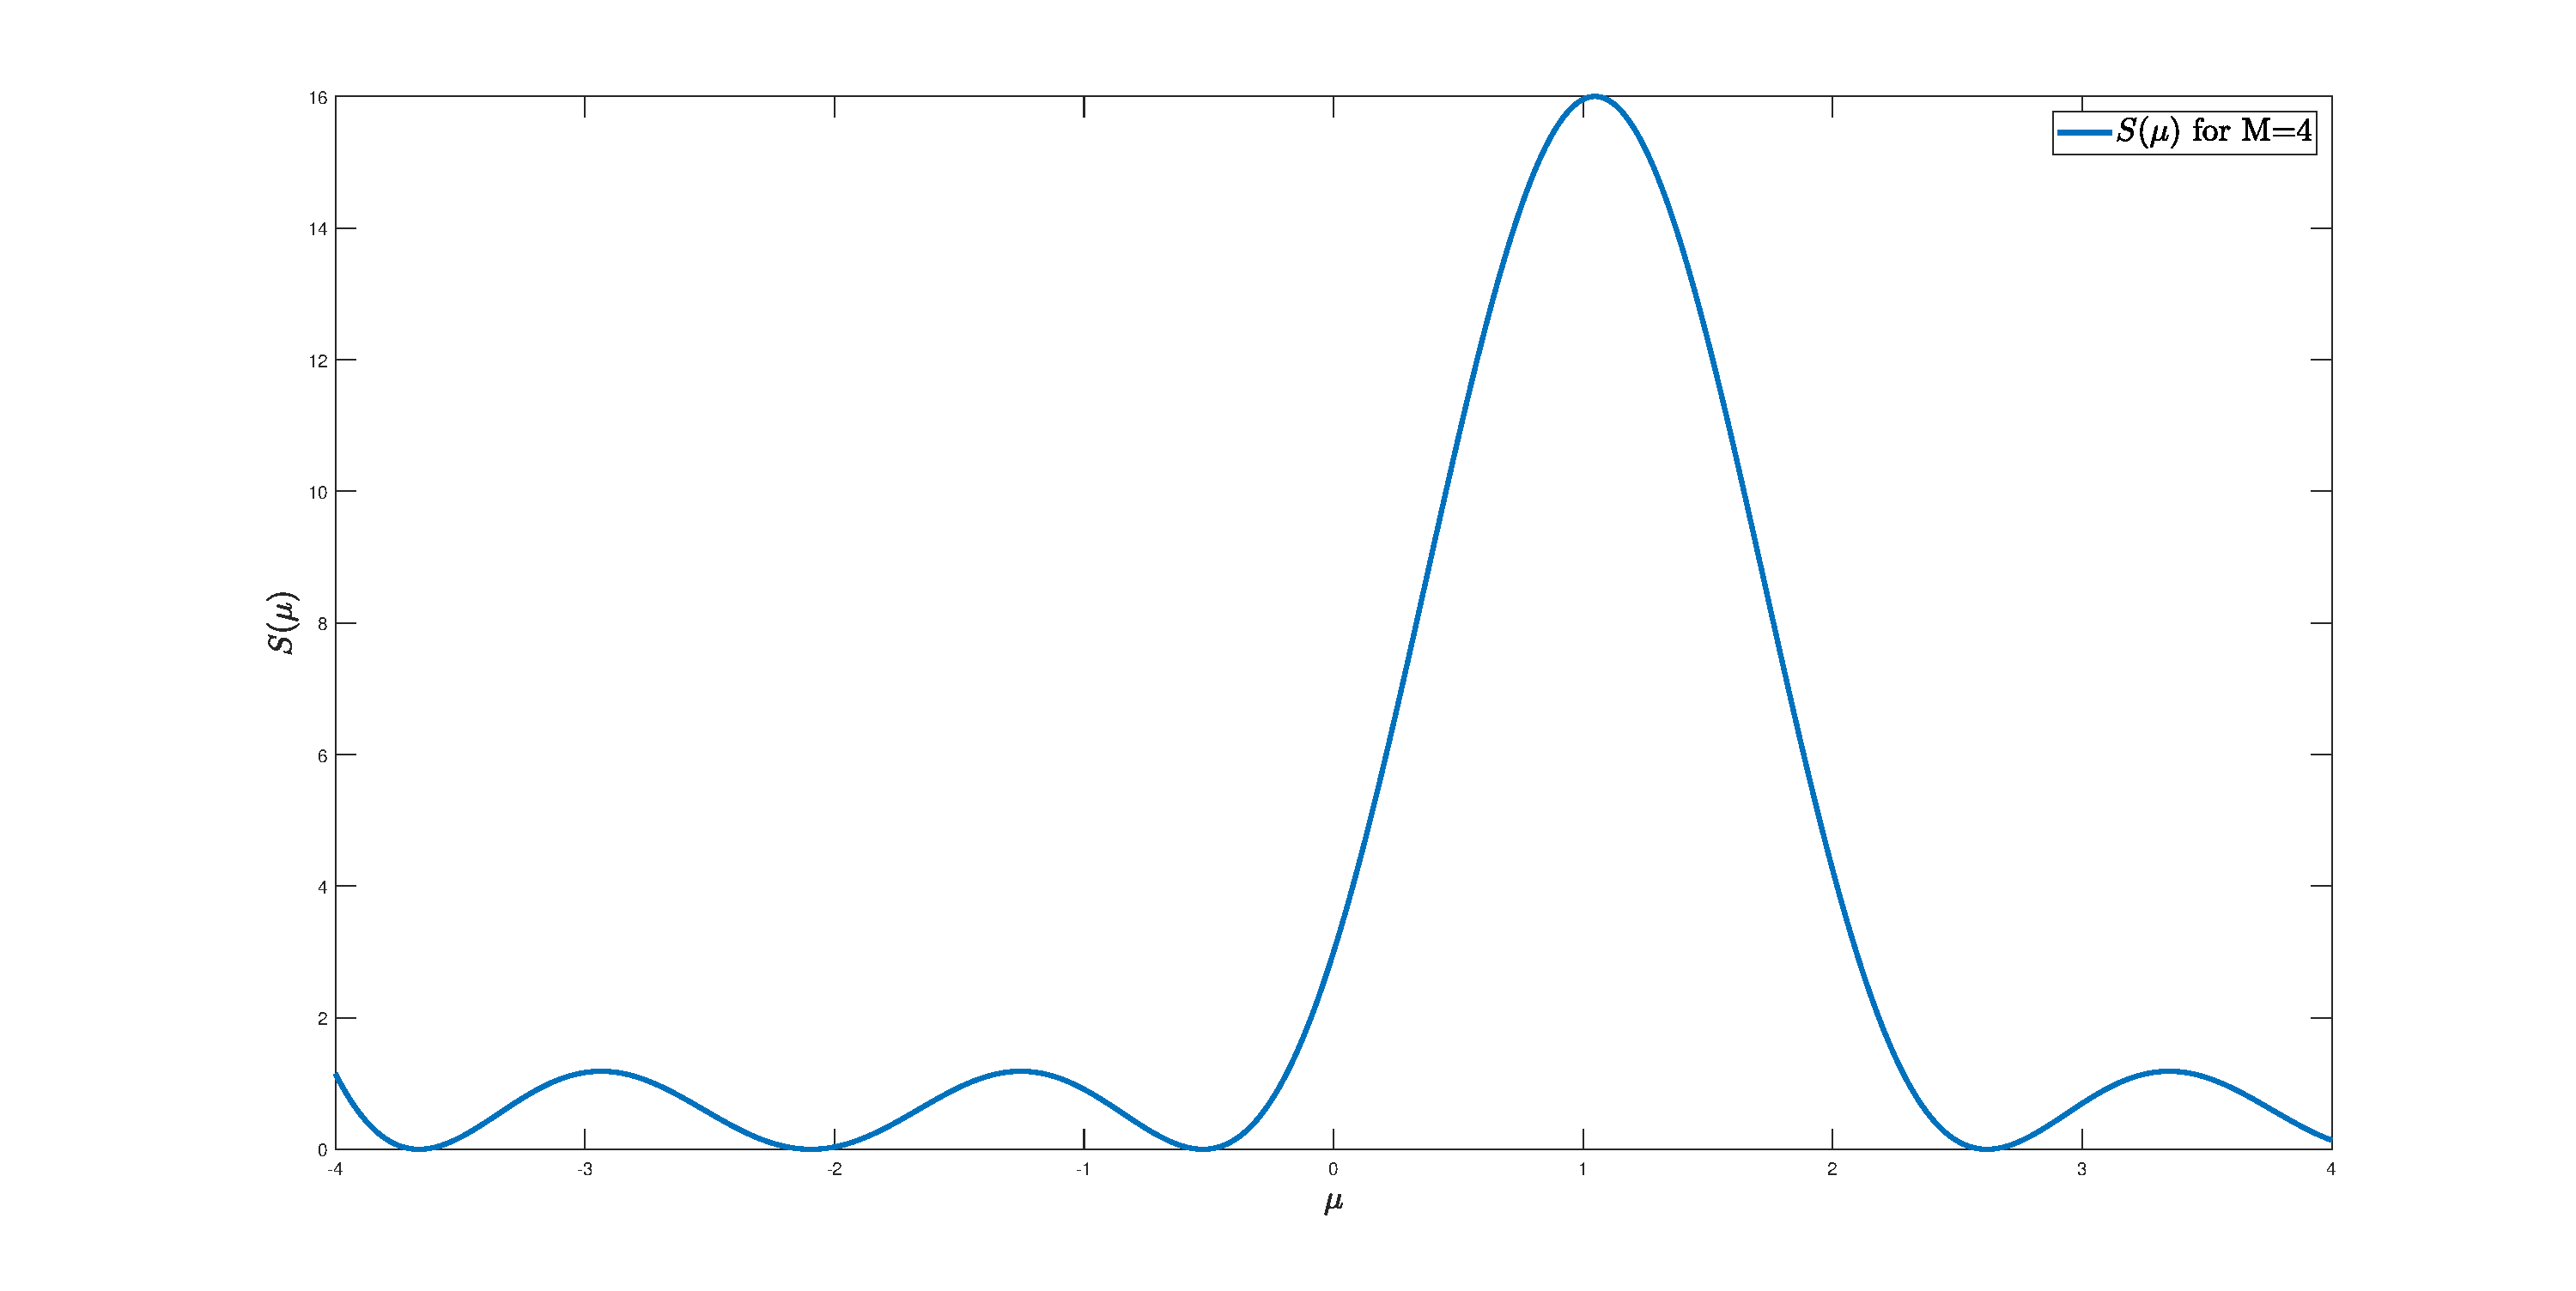
\includegraphics[trim =3cm 1cm 3cm 0cm, clip, width=1.00\textwidth]{graphics/Space_Spectrum_Analyzer_M_4.pdf}
	\caption{Fourier Periodogram for four sensors ($M=4$)}
	\label{fig:Space_Spectrum_Analyzer_M_4}
\end{figure}

\begin{figure}[H]
	\centering
		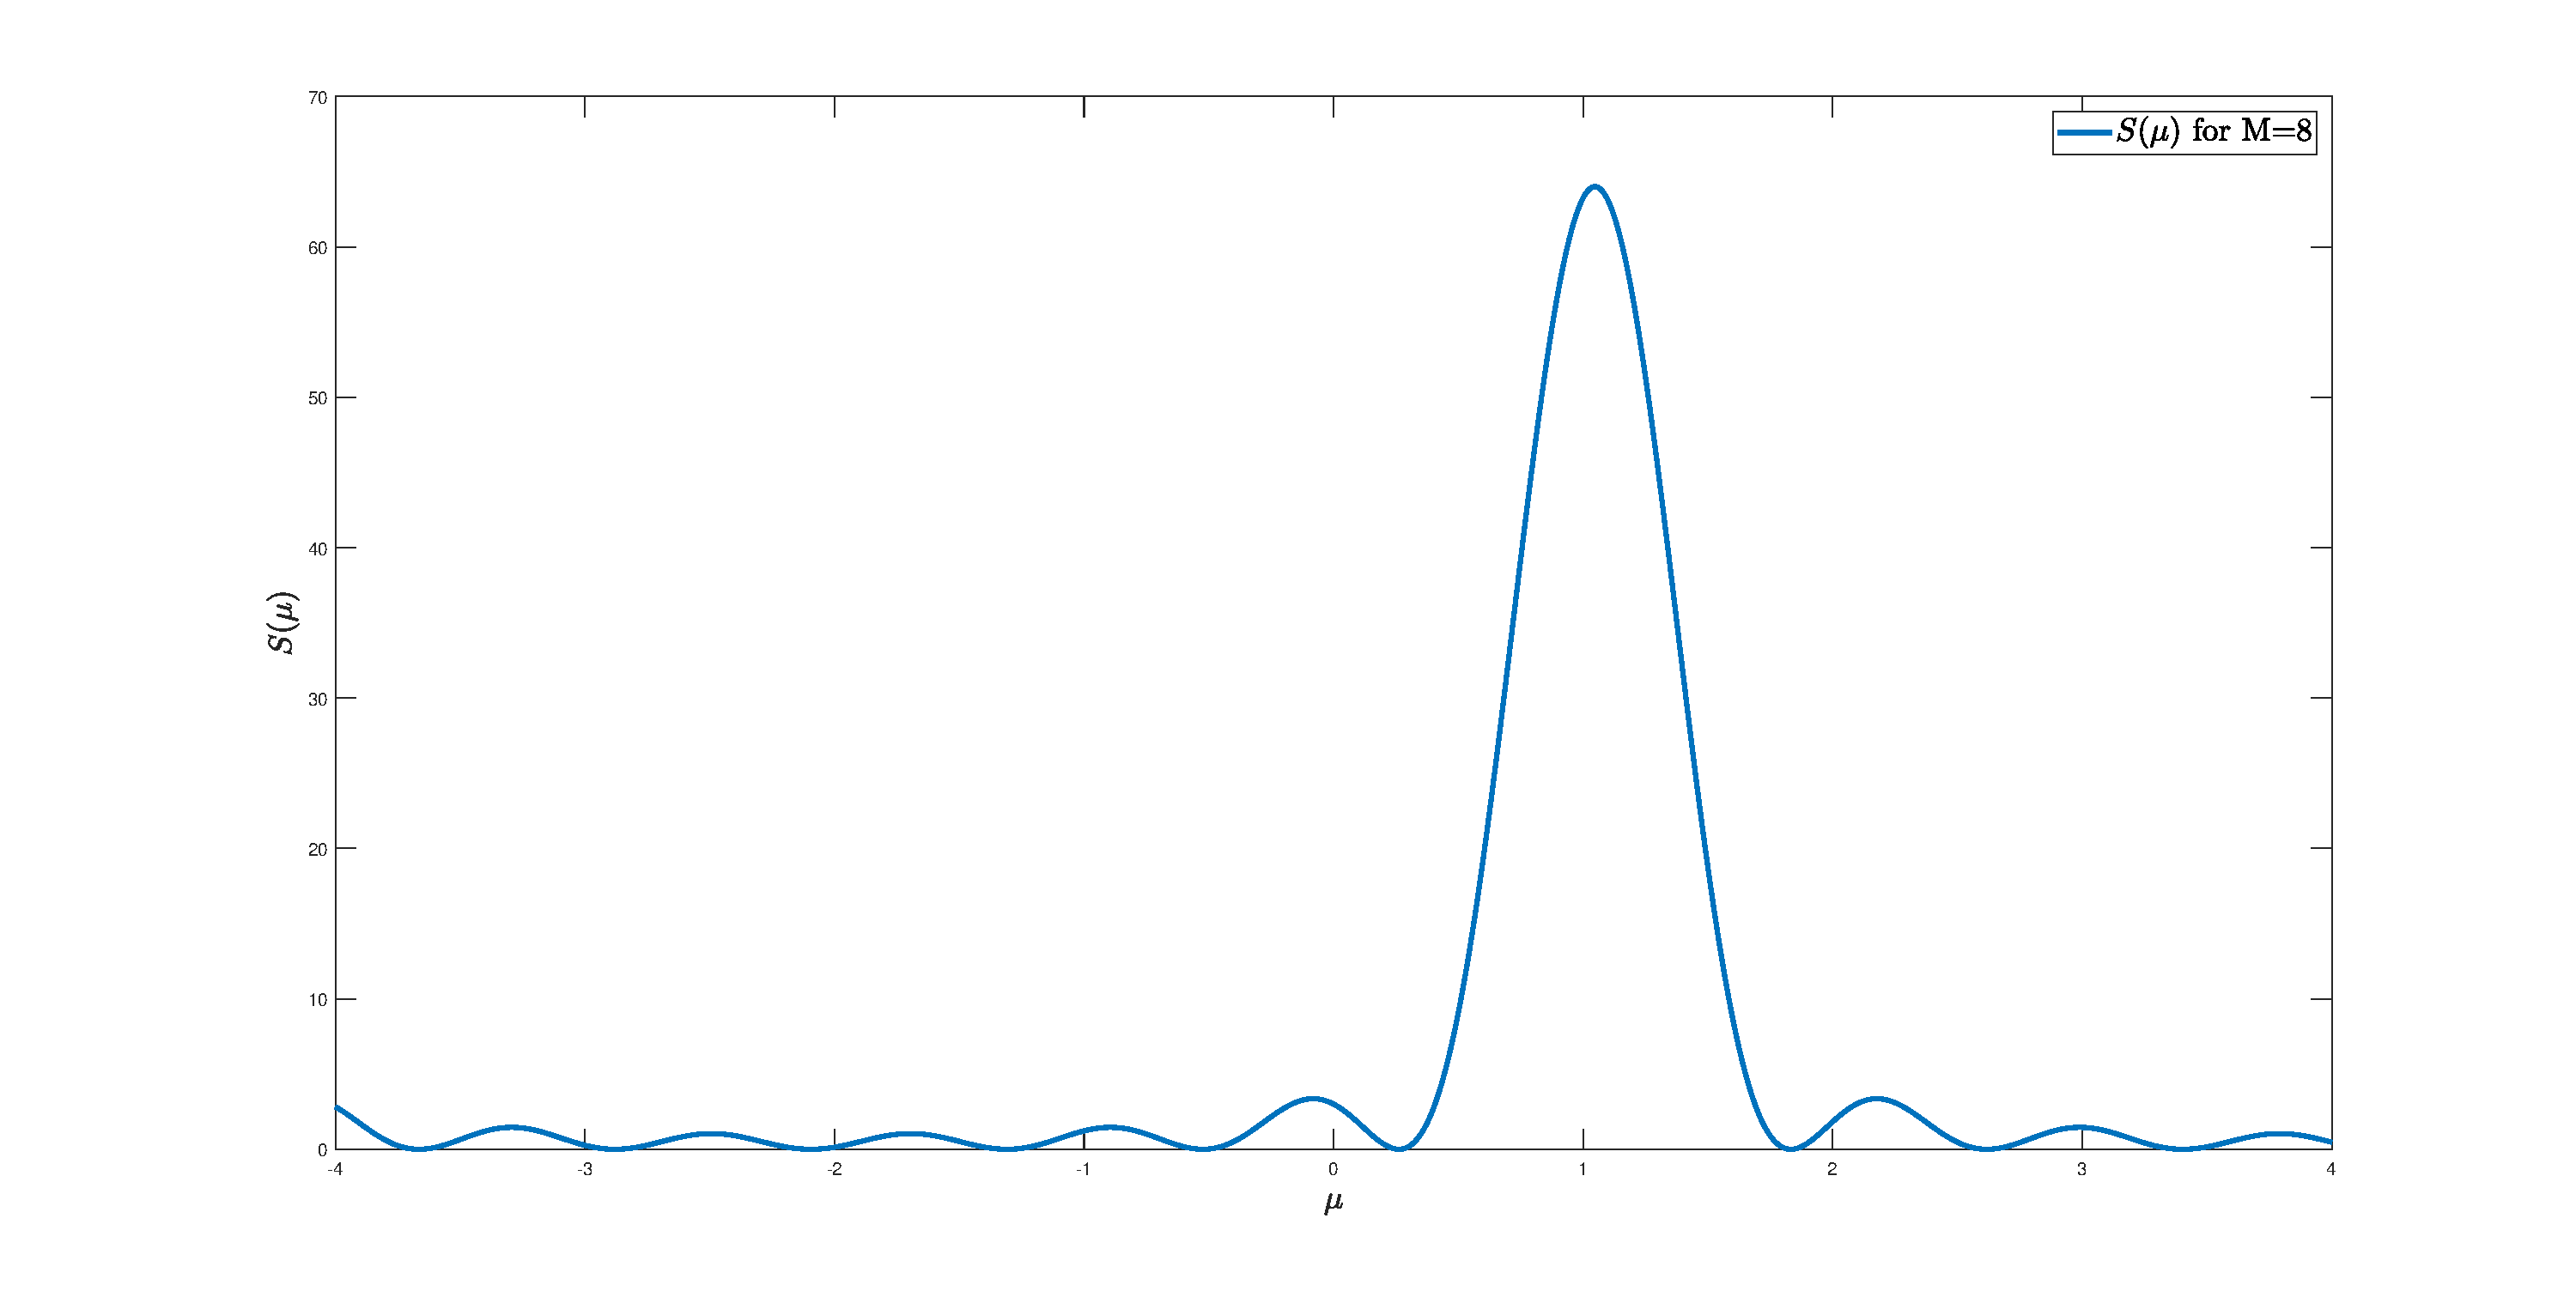
\includegraphics[trim =3cm 1cm 3cm 0cm, clip, width=1.00\textwidth]{graphics/Space_Spectrum_Analyzer_M_8.pdf}
	\caption{Fourier Periodogram for eight sensors ($M=8$)}
	\label{fig:Space_Spectrum_Analyzer_M_8}
\end{figure}

As can be seen from figures \ref{fig:Space_Spectrum_Analyzer_M_4} and \ref{fig:Space_Spectrum_Analyzer_M_8} the resolution is limited. This limit (space between maximum and next zero) is called "Rayleigh-limit" ($\Delta\mu$) and depends on the number of sensors $M$ as follows:\\
$\Delta\mu=\frac{2\pi}{M}$\\
The only way to increase the resolution (decrease "Rayleigh-limit" $\Delta\mu$) is to increase the number of sensors. However this leads to higher costs. Therefore it is not our preferred solution.\\ 
Can we do better?\\ \ \\
\begin{tabular}{ll}
\Ra& Yes, e. g. by using the MVDR (minimum variance distortion-less response) spectrum estimation:\\
 & $S_{MVDR}(\mu)=\frac{1}{\vec{a}^H(\mu)\ma{\hat{R}}_x^{-1}\vec{a}(\mu)}$\\
 & $S_{FPG}(\mu)=\vec{a}^H(\mu)\ma{\hat{R}}_x\vec{a}(\mu)\qquad $ Where FPG stands for Fourier Periodogram (for comparison)\\
\end{tabular}

For \underline{zero noise} the MVDR-spectrum has \underline{no} resolution limitation!\\ 
The MVDR is the same algorithm as the Digital spectrum analyser (\autoref{sssec:dsa}) but with the spatial sampling.
\\ \ \\
Can we do better?\\
\begin{tabular}{ll}
\Ra& Yes, trade-off of SNR with number $N$ of snapshots taken:\\
&$\rightarrow$ \underline{MUSIC}-spectrum:\\
& Resolution depends on $N\cdot SNR$ besides on $M$\\
\end{tabular}
\newpage
\subsection{MUSIC-Algorithm (Multiple Signal Classification)}
\textit{
\begin{center}
"Music was my first love\\
And it will be last."
\end{center}}

Processing the signals received on an array of sensors for the location of the emitter is of great enough interest to have been treated under many special case assumptions. The general problem considers sensors with arbitrary locations and arbitrary directional characteristics (gain/phase/polarization) in a noise interference environment of arbitrary covariance matrix. The \textbf{mu}ltiple \textbf{si}gnal \textbf{c}lassification (MUSIC) algorithm provides asymptotically unbiased estimates of
\begin{enumerate}
	\item number of incident wavefronts present
	\item directions of arrival (DOA) (or emitter locations)
	\item strengths and cross correlations among the incident waveforms
	\item noise/interference strength\cite{Schmidt:MUSIC}
\end{enumerate}

$\vec{x}[n]=\ma{A}\vec{s}[n]+\vec{\nu}[n]$\\
\begin{flalign*}
\ma{A}&=\mat{\vec{a}(\mu_1)& \vec{a}(\mu_2) & \shdots & \vec{a}(\mu_d)}, \qquad \rank\ma{A}=d \pfeil \textrm{steering vectors are LID}&&\\
&=\ma{U}\ma{\Sigma}\ma{V}^H\qquad \text{(SVD)}
\end{flalign*}

$\ma{U}=\mat{\vec{u}_1 & \vec{u}_2 & \shdots & \vec{u}_d & \vec{u}_{d+1} & \vec{u}_{d+2} &\shdots & \vec{u}_M}$\\
We can partition \ma{U} into the two matrices $\ma{U}_1$ and $\ma{U}_2$ ($\ma{U}=\mat{\ma{U}_1 & \ma{U}_2}$) with\\
$\ma{U}_1 = \mat{\vec{u}_1 & \vec{u}_2 & \shdots & \vec{u}_d}$\\
and
$\ma{U}_2 = \mat{\vec{u}_{d+1} & \vec{u}_{d+2} &\shdots & \vec{u}_M}$\\ \\

Recall the properties of matrices from the SVD:\\
$\ma{U}^H_1\ma{U}_1=\ma{I}, \qquad \ma{U}^H_2\ma{U}_2=\ma{I}, \qquad \ma{U}^H_1\ma{U}_2=\ma{0}, \qquad \ma{U}^H_2\ma{U}_1=\ma{0}$\\
$\ma{U}_1\ma{U}^H_1 + \ma{U}_2\ma{U}^H_2 = \ma{I}$\\
$\text{im}\ma{A}= \text{im}\ma{U}_1 \pfeil
\left\lbrace \begin{matrix}
 \forall \mu\in\{\mu_1,\mu_2,\ldots,\mu_d\}:\, \vec{a}(\mu)\in\text{im}\ma{A}\\
 \forall \mu\in\{\mu_1,\mu_2,\ldots,\mu_d\}:\exists\vec{x}:\vec{a}(\mu)=\ma{U}_1\vec{x}
\end{matrix} \right.$\\
Therefore\\
$\ma{U}_2^H\vec{a}(\mu_i)=\underbrace{\ma{U}_2^H\ma{U}_1}{=\ma{0}}\vec{x}=\vec{0}$\\ \ \\

\subsubsection{Ideal MUSIC spectrum}

$S_{\text{MUSIC, IDEAL}}(\mu)=\frac{||\vec{a}(\mu)||_2^2}{||\ma{U}_2^H\vec{a}(\mu)||_2^2}$\\
We assume that $\vec{a}(\mu)\neq0$ holds for any $\mu$.\\ \\

To compute the actual spectrum we divide the $\mu$s into two parts.\\ \\

\textbf{Case 1:}\\
Lets start with $\mu\in\{\mu_1,\ldots,\mu_d\}$:
As we derived above $\ma{U}_2^H\vec{a}(\mu_i)=0$ and therefore it's Euclidean norm is also zero. So we get:\\
$\Rightarrow S_{\text{MUSIC, IDEAL}}(\mu_i)=\infty$\\

\textbf{Case 2:}\\
Assume: $\mat{\vec{a}(\mu_1)& \vec{a}(\mu_2) & \shdots & \vec{a}(\mu_d) & \vec{a}(\mu)}$ are L. I. D. with $\mu\notin\{\mu_1,\ldots,\mu_d\}$.\\
$\vec{a}(\mu)\notin\text{im}\ma{A}=\text{im}\ma{U}_1$\\
$\vec{a}(\mu)\in\text{im}\ma{U}_2$\\
$\vec{a}(\mu)=\ma{U}_2\cdot\vec{y};\qquad \vec{y}\in\mathbb{C}^{(M-d)\times 1};\qquad M-d\geq1$\\
\mybox{
Out of this we get the restriction that the number of sensors must be at least one more than the number of arriving wavefronts:\\
$d\leq M-1$
}
$\ma{U}_2^H\vec{a}(\mu)=\underbrace{\ma{U}_2^H\ma{U}_2}{\ma{I}}\vec{y}=\vec{y}\neq\vec{0}$\\
$\Rightarrow S_{\text{MUSIC, IDEAL}}(\mu)<\infty$ for $\mu\notin\{\mu_1,\ldots,\mu_d\}$\\ \ \\

Summarizing both cases we get:\\
$S_{\text{MUSIC, IDEAL}}(\mu)=\left\lbrace \begin{matrix}\infty,& \text{for} \mu\in\{\mu_1,\ldots,\mu_d\}\\<\infty,&\text{else}\end{matrix} \right.$\\ \ \\

\begin{figure}[H]
	\centering
		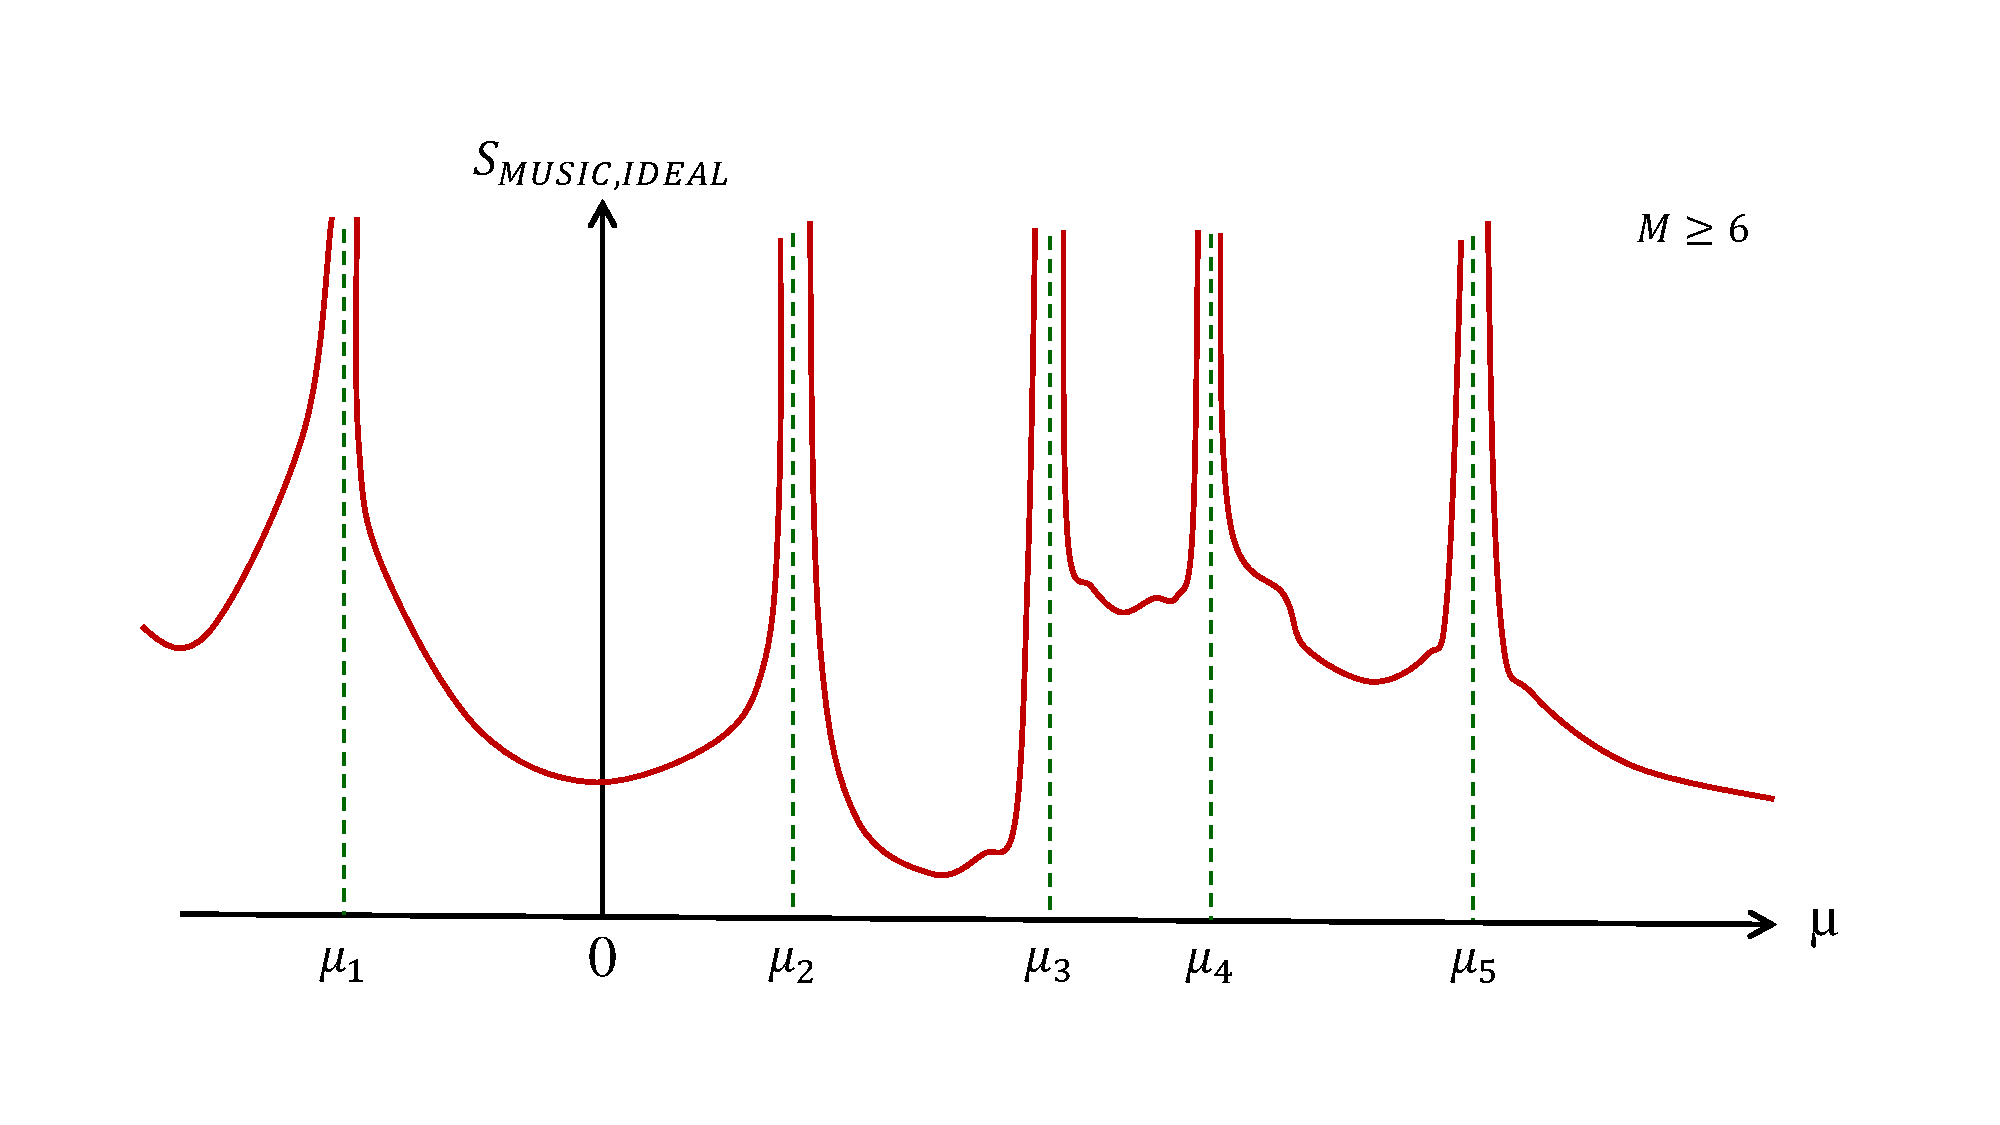
\includegraphics[trim =2cm 2cm 2cm 2cm, clip, width=0.90\textwidth]{graphics/Ideal_MUSIC_spectrum.pdf}
	\caption{Ideal MUSIC spectrum \Ra no resolution limit!}
	\label{fig:Ideal_MUSIC_spectrum}
\end{figure}
As we can see in figure \ref{fig:Ideal_MUSIC_spectrum} there is no resolution limit in the ideal music spectrum. We can be as precise as necessary.

\subsubsection{Problems with the MUSIC spectrum}
However we got 2 problems:
\begin{enumerate}
	\item $\mat{\vec{a}(\mu_1)& \vec{a}(\mu_2) & \shdots & \vec{a}(\mu_d) & \vec{a}(\mu)}$ may L. D.
	\item We don't know $\ma{U}_2$ because \ma{A} is unknown 
\end{enumerate}

\paragraph{Problem 1: Linear dependence of steering vectors}
Let's first look a bit deeper into problem 1:\\
Intuitively it create linear dependent steering vectors (\vec{a}) seems only possible if we place the sensors (antennas) in a well-arranged structure. So we consider an uniform linear array (ULA) that is such a structure.\\
$\vec{a}(\mu_1)=\mat{1\\a\\a^2},\qquad\vec{a}(\mu_2)=\mat{1\\b\\b^2},\vec{a}(\mu)=\mat{1\\c\\c^2}$\\
where $a=e^{\j\mu_1},\quad b=e^{\j\mu_2},\quad c=e^{\j\mu}$ and $a\neq b,\quad a\neq c, b\neq c$\\
$\mat{1&1&1\\a&b&c\\a^2&b^2&c^2}\mat{\alpha\\\beta\\\gamma}=\vec{0}$\\
In order to solve this set of linear equations we use the Gaussian elimination:\\
$\mat{1&1&1\\0&a-b&a-c\\0&a^2-b^2&a^2-c^2}\mat{\alpha\\\beta\\\gamma}=\mat{0\\0\\0}$\\
$\mat{1&1&1\\0&a-b&a-c\\0&0&(c-b)(a-c)}\mat{\alpha\\\beta\\\gamma}=\mat{0\\0\\0}$\\
Since $(c-b)(a-c)\neq 0$ we get:\\
$\gamma=0$\\
The same happens for $\beta$ and $\alpha$:\\
$\underbrace{(a-b)}_{\neq 0} \beta = 0 \Ra \beta=0$\\
$\alpha=0$\\
This means, that even for an ULA we get L. I. D steering vectors if $\Delta<\frac{\lambda}{2}$.\\
It turns out that it is quiet hard to place the sensors such that the steering vectors are L. D.  So in general problem 1 does not affect us in most of the cases.

\paragraph{Problem 2: Determine the steering matrix A}
Recall the singular value decomposition (SVD) of matrix \ma{A}:
$\ma{A}=\ma{U}\ma{\Sigma}\ma{V}^H$\\
$\ma{A}\ma{R}_s\ma{A}^H=\ma{U}\underbrace{\ma{\Sigma}\ma{V}^H\ma{R}_s\ma{V}\ma{\Sigma}^T}_{\ma{\Lambda}}\ma{U}^H=\ma{U}\ma{\Lambda}\ma{U}^H$\\
Where $\ma{\Lambda}$ is the eigenvalue matrix.\\
Now let's assume $\ma{R}_s$ has full rank, which means $\rank\ma{R}_s=d$. Therefore the eigenvalue decomposition (EVD) of $\ma{R}_s$ exists and is given as follows:\\
$\ma{R}_s=\ma{Q}\ma{\Lambda}'\ma{Q}^H;\qquad \ma{\Lambda}'>\vec{0}$ (positive definite)\\
$\ma{R}_s^{\frac{1}{2}}=\ma{Q}\ma{\Lambda}'^{\frac{1}{2}}\ma{Q}^H$\\
Since $\ma{\Lambda}'^{\frac{1}{2}}$ is real valued we can conclude: $\left(\ma{R}^{\frac{1}{2}}\right)^H=\ma{R}^{\frac{1}{2}}$\\
$\ma{A}\ma{R}_s\ma{A}^H=\ma{A}\ma{R}^{\frac{1}{2}}\ma{R}^{\frac{1}{2}}\ma{A}^H=\underbrace{\ma{A}\ma{R}^{\frac{1}{2}}}_{\ma{G}}\underbrace{\left(\ma{R}^{\frac{1}{2}}\right)^H\ma{A}^H}_{\ma{G}^H}=\ma{G}\ma{G}^H$\\
$\Ra \ma{A}\ma{R}_s\ma{A}^H$ turns out to be a Gramian matrix (see section \ref{sec:Gramian_matrix}).\\
\begin{flalign*}
\text{im}\ma{A}\ma{R}_s\ma{A}^H&=\text{im}\ma{G}\ma{G}^H&&\\
&=\text{im}\ma{A}\ma{R}^{\frac{1}{2}}&&\\
&=\text{im}\ma{A}\qquad \text{since } \ma{R}^{\frac{1}{2}} \text{ is invertible}
\end{flalign*}
$\text{im}\ma{A}=\left\lbrace\ma{A}\vec{x}\left.\right|\vec{x}\in\mathbb{C}^{d\times 1}\right\rbrace$\\
$\text{im}\ma{A}\ma{R}^{\frac{1}{2}}=\left\lbrace\ma{A}\underbrace{\ma{R}^{\frac{1}{2}}\vec{y}}_{=\vec{x}}\left.\right|\vec{y}\in\mathbb{C}^{d\times 1}\right\rbrace$\\
Note: $\vec{x}=\ma{R}^{\frac{1}{2}}\vec{y} \Ra \vec{y}=\ma{R}^{-\frac{1}{2}}\vec{x}$\\
$\rank\ma{A}\ma{R}_s\ma{A}^H=\rank\ma{A}=d$\\
$\ma{A}\ma{R}_s\ma{A}^H=\ma{U}\ma{\Lambda}\ma{U}^H=\mat{\ma{U}_1&\ma{U}_2}\mat{\lambda_1& & & & & & \\ &\lambda_2 & & & & &\\ & &\ddots& & & &\\ & & &\lambda_d& & &\\ & & & & 0& &\\ & & & & & \ddots& \\& & & & & &0}\mat{\ma{U}_1^H\\\ma{U}_2^H}$\\
$\vec{x}[n]=\ma{A}\vec{s}[n]+\vec{\nu}[n]$\\
If we assume that noise and signal are uncorrelated (what usually is the case)  we get the following:\\
\mybox{
$E\left[\vec{x}[n]\vec{x}^H[n]\right]=\ma{R}_x=\ma{A}\ma{R}_s\ma{A}^H+\ma{R}_\nu$}\\
Note that $E\left[\vec{x}[n]\vec{x}^H[n]\right]$ can be estimated from array observations.\\
$\ma{\hat{R}}_x=\frac{1}{N}\ma{X}\ma{X}^H$\\
To make things easier we assume the noise to be white which means $\ma{R}_\nu=\sigma_\nu^2\ma{I}$. So we get:\\
\begin{flalign*}
\ma{R}_x&=\underbrace{\ma{A}\ma{R}_s\ma{A}^H}_{\ma{U}\ma{\Lambda}\ma{U}^H}+\sigma_\nu^2\underbrace{\ma{I}}_{\ma{U}\ma{U}^H}&&\\
&=\ma{U}\underbrace{(\ma{\Lambda}+\sigma_\nu^2\ma{I})}_{=\ma{\Lambda}'}\ma{U}^H
\end{flalign*}
\mybox{
$\ma{R}_x=\ma{U}(\ma{\Lambda}+\sigma_\nu^2\ma{I})\ma{U}^H=\ma{U}\ma{\Lambda}'\ma{U}^H$
}

If we sort the eigenvalues such that $\lambda_1\geq\lambda_2\geq\ldots\geq\lambda_d>0$ we get the following eigenvalue matrix $\ma{\Lambda}'$:\\
$\ma{\Lambda}'=\mat{\lambda_1+\sigma_\nu^2& & & & & & \\ &\lambda_2+\sigma_\nu^2 & & & & &\\ & &\ddots& & & &\\ & & &\lambda_d+\sigma_\nu^2& & &\\ & & & & \sigma_\nu^2& &\\ & & & & & \ddots& \\& & & & & &\sigma_\nu^2}$\\

$\lambda_k'=\lambda_k+\sigma_\nu^2$: Eigenvalue of $\ma{R}_x$

\begin{figure}[H]
	\centering
		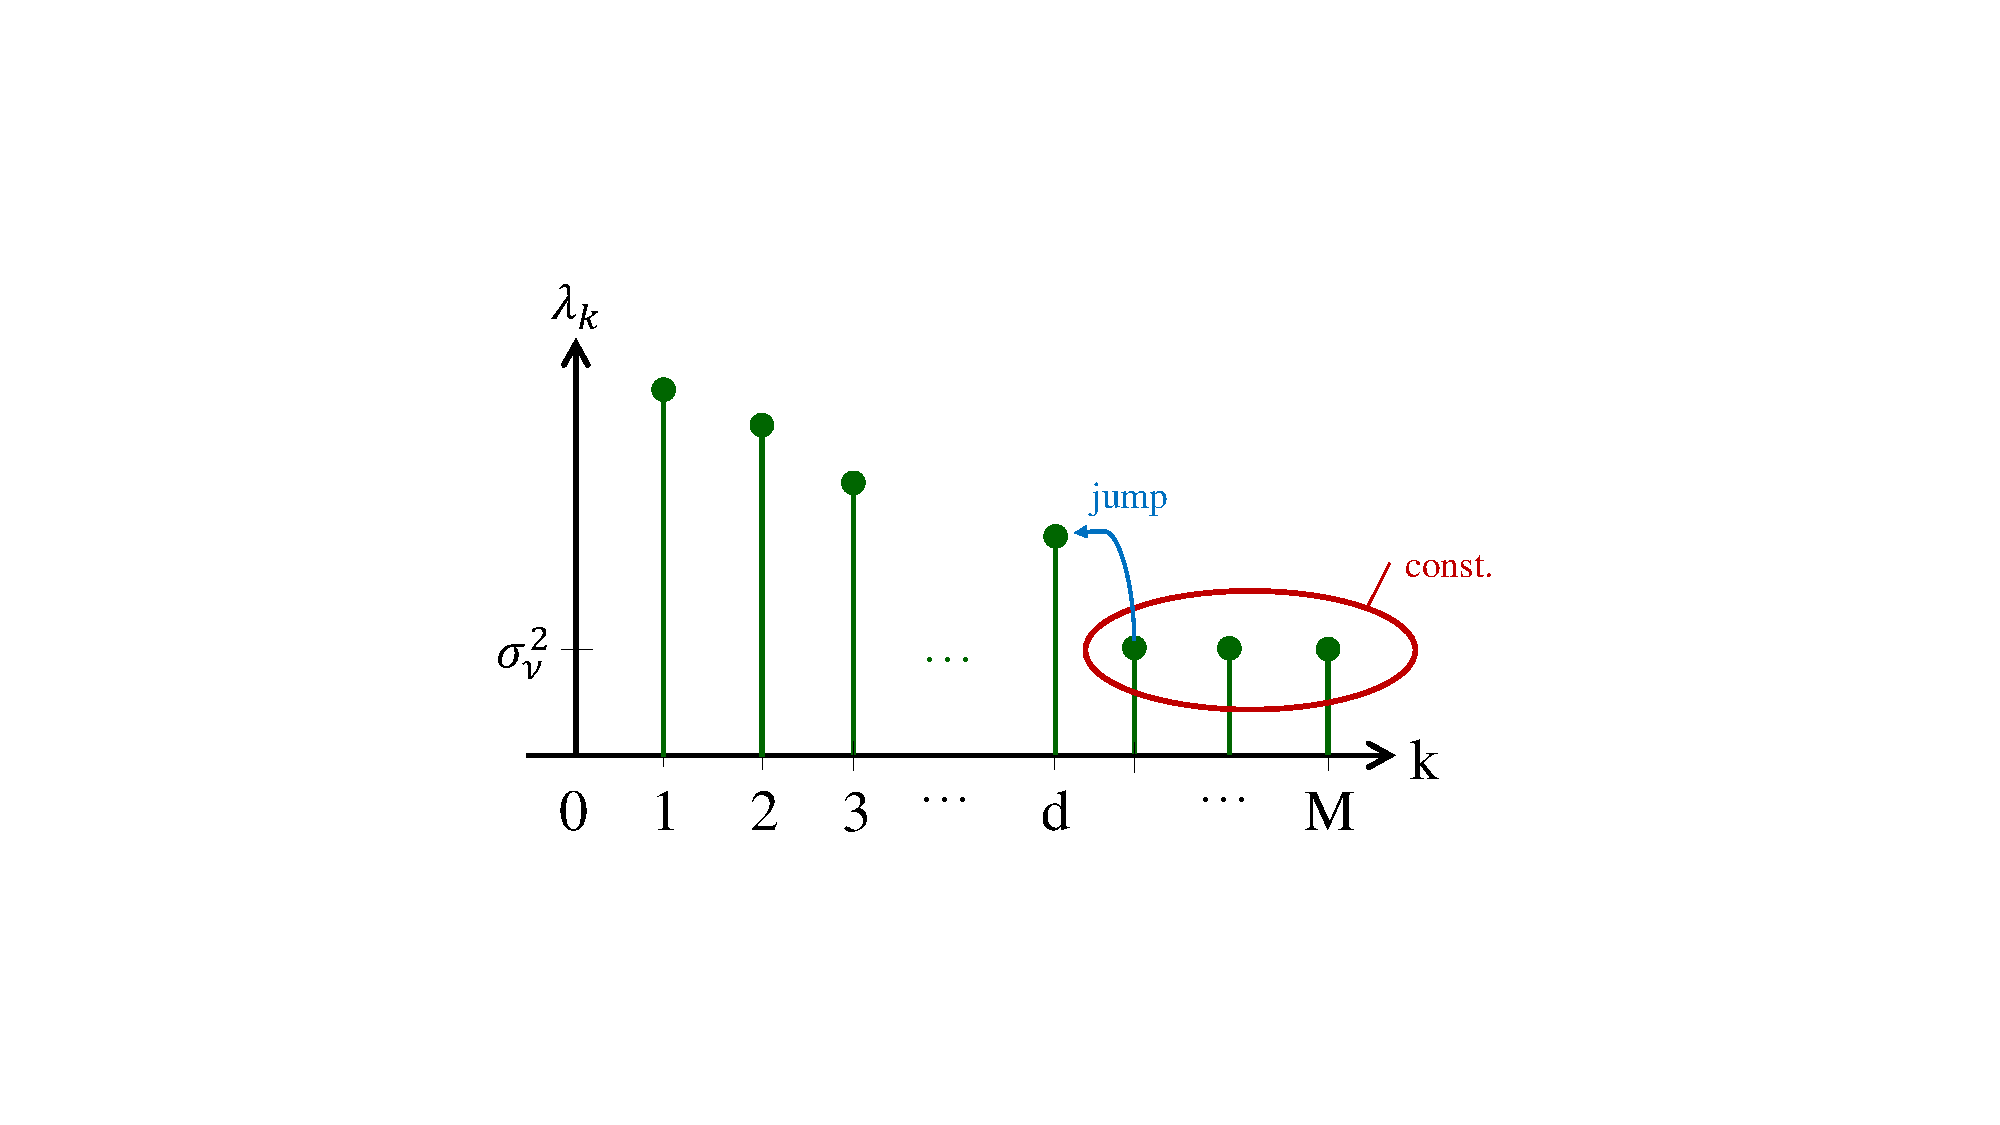
\includegraphics[trim =5cm 5cm 5cm 4cm, clip, width=0.80\textwidth]{graphics/Ideal_MUSIC_eigenvalues.pdf}
	\caption{Ideal (all noise EVs have the same height) eigenvalue spectrum for MUSIC}
	\label{fig:Ideal_MUSIC_eigenvalues}
\end{figure}

From the picture, we get d and can determine $\ma{U}_2$:\\
$\ma{U}_2=\mat{\vec{u}_{d+1}&\vec{u}_{d+1}&\shdots&\vec{u}_{M}}$\\
$\ma{R}_x$ is still unknown but we can take $\ma{\hat{R}}_x$ in its place:\\
$\ma{\hat{R}}_x=\frac{1}{N}\sum\limits_{k=0}^{N-1}\vec{x}[n+k]x^H[n+k]=\frac{1}{N}\ma{X}\ma{X}^H$\\
$\ma{X}=\mat{\vec{x}[n]&\vec{x}[n+1]&\shdots&\vec{x}[n+N-1]}$\\

\begin{figure}[H]
	\centering
		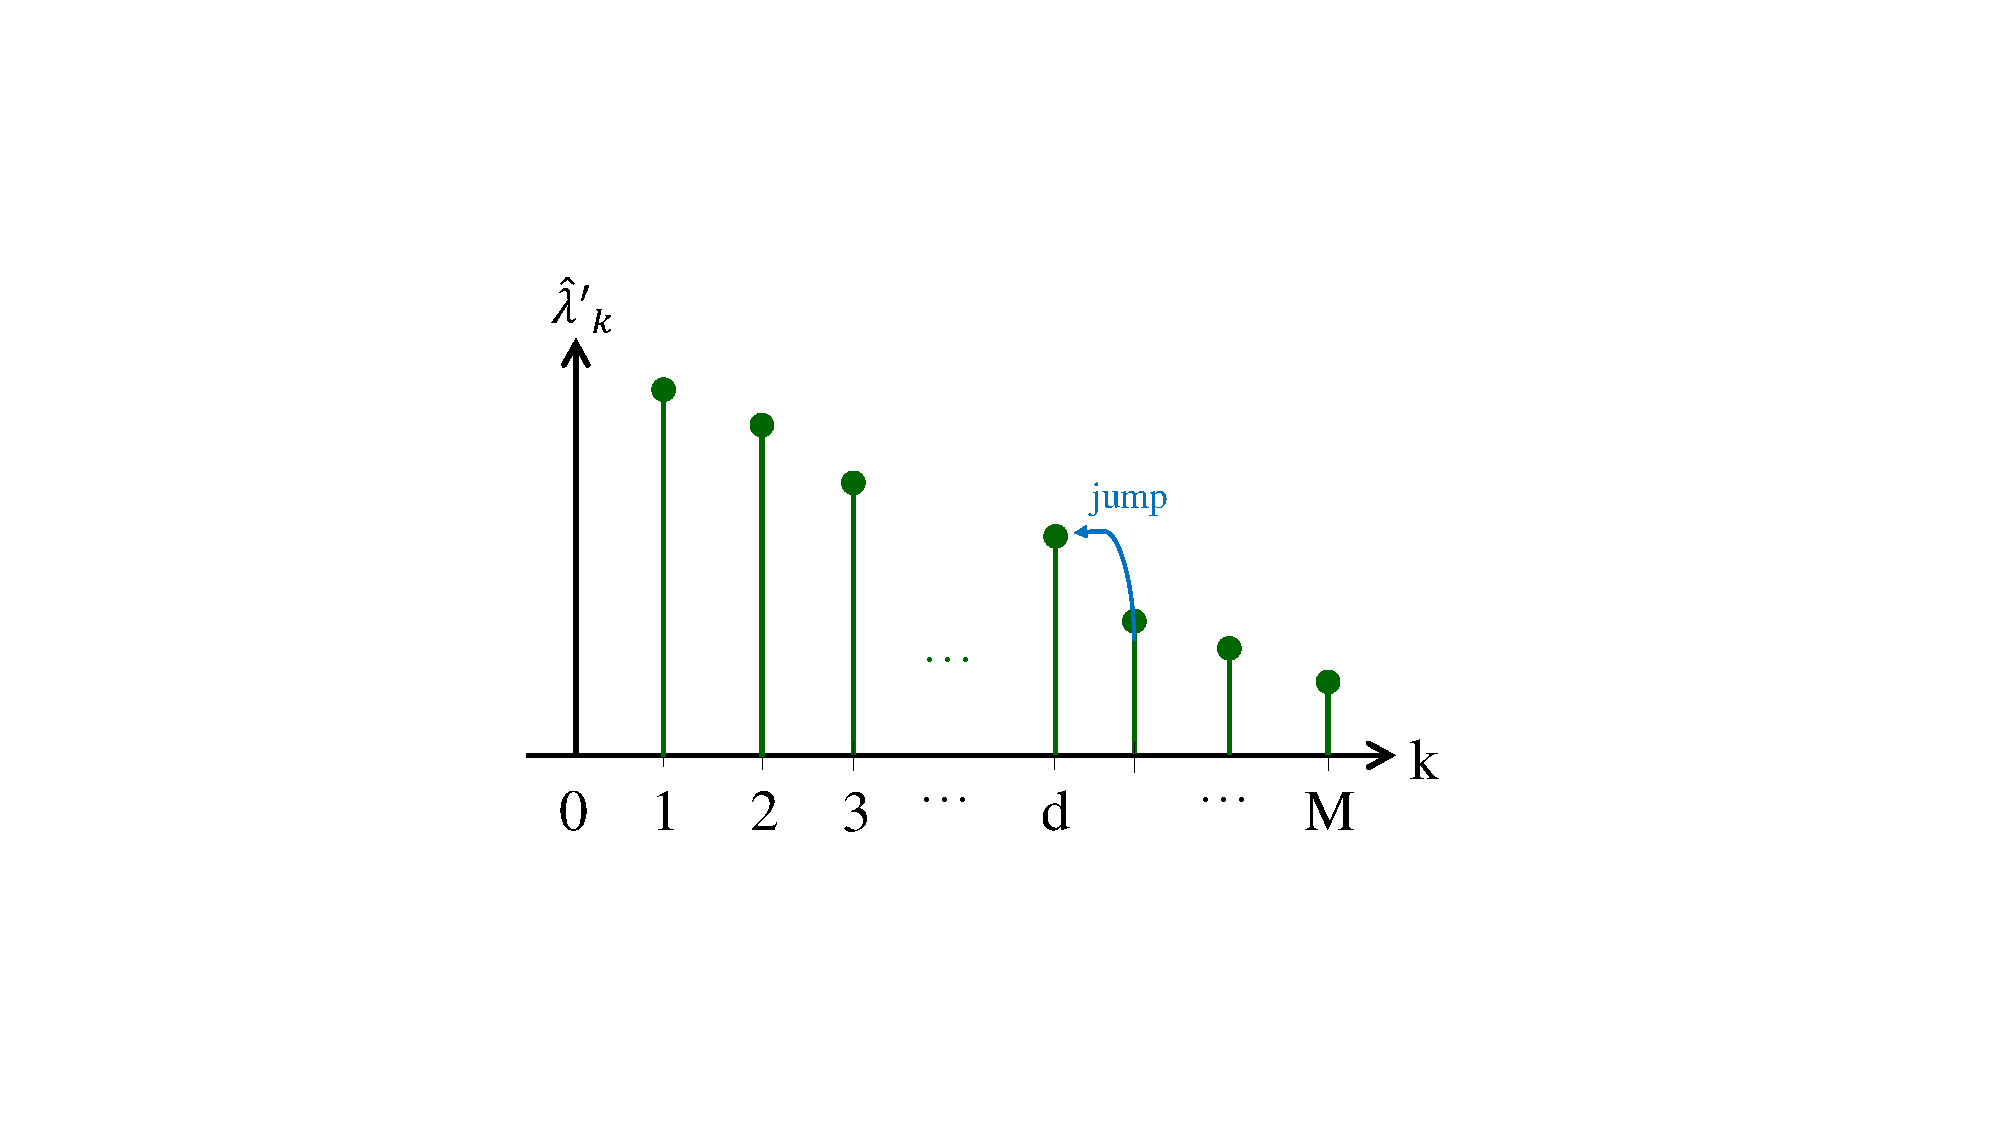
\includegraphics[trim =5cm 5cm 5cm 4cm, clip, width=0.80\textwidth]{graphics/Real_MUSIC_eigenvalues.pdf}
	\caption{Real (noise EVs have NOT the same height) eigenvalue spectrum for MUSIC}
	\label{fig:Real_MUSIC_eigenvalues}
\end{figure}

\newpage
\paragraph{Jump detection}
As can be seen above a jump detection is needed in order to determine the number of arriving wavefronts $d$. This can be done by defining a threshold $q$. If the difference between the m-th eigenvalue and the (m-1)-st is larger than this threshold this is considered as jump and the value for $d$ is found. But now the question is how to set $q$ such that it is neither to small nor to big.\\

\begin{figure}[H]
	\centering
		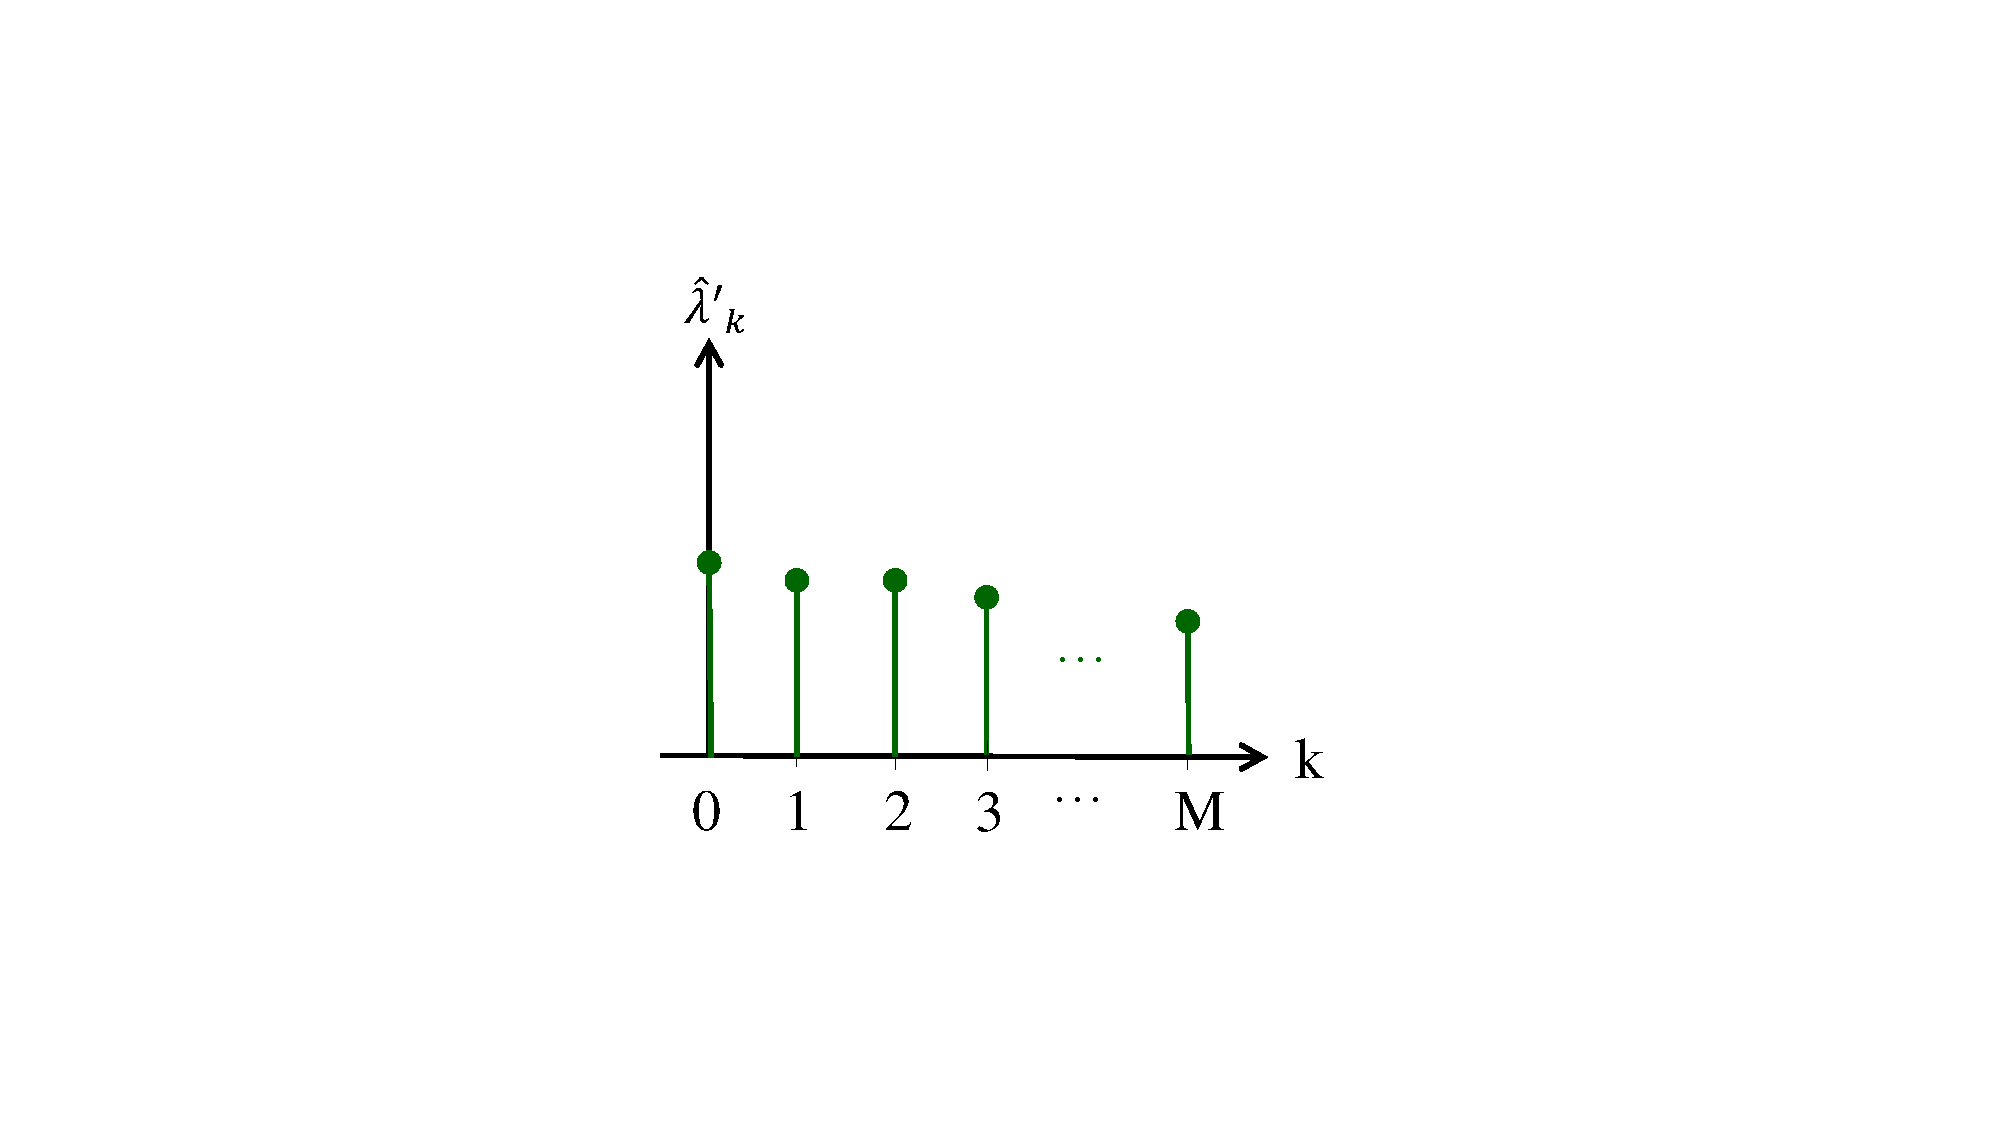
\includegraphics[trim =5cm 5cm 5cm 4cm, clip, width=0.80\textwidth]{graphics/jump_detection_noise.pdf}
	\caption{Noise eigenvalues to determine the minimum jump size $q$}
	\label{fig:jump_detection_noise}
\end{figure}

Let's assume that $d=0$ so we got pure noise. Then we define a probability $p$ of identifying the wrong  $q$:\\

$p=P_r\left[\frac{\hat{\lambda}'_m}{\hat{\lambda}'_{m-1}}>q\right]$\\
After that a Monte-Carlo-Experiment can be run. Out of this experiment jump sizes $q$ can be determined (see table \ref{tab:min_step_size_q}).\\
\begin{table}[H]
\begin{center}
\begin{tabular}{lc|c|c|c}
Sensors&$M$&4&8&8\\
\hline
Snapshots&$N$&100&10&1000\\
\hline
Probability&$p$&0.01&0.01&0.01\\
\hline
Threshold&$q$&\textcolor[rgb]{1,0,0}{1.45}&\textcolor[rgb]{1,0,0}{1.34}&\textcolor[rgb]{1,0,0}{1.09}\\
\end{tabular}
\end{center}
\caption{Results for minimum jump size $q$ (Monte-Carlo-experiment)}
\label{tab:min_step_size_q}
\end{table}

\mybox{
\subsubsection{Summary: MUSIC-Algorithm}
\textbf{Input:} $\ma{X}\in\mathbb{C}^{M\times N};\qquad M=\text{number of sensors},\qquad N=\text{number of snapshots}$\\
\textbf{Output:} $\mu_1,\,\mu_2,\,\ldots,\,\mu_{\hat{d}},\hat{d}$\\
\textbf{Assume white noise!}\\
\begin{enumerate}
	\item $\ma{\hat{R}}_x=\frac{1}{N}\ma{X}\ma{X}^H$ (maximum likelihood estimation for Gauss'ian noise)
	\item EVD: $\ma{\hat{R}}_x=\ma{\hat{U}}\ma{\hat{\Lambda}}'\ma{\hat{U}}^H$
	\item Estimate d: ``Jump detection''
	\item 	Partition $\ma{\hat{U}}$:\\
				$\ma{\hat{U}}=\mat{\vec{\hat{u}}_1&\shdots&\vec{\hat{u}}_{\hat{d}}&\vec{\hat{u}}_{\hat{d}+1}&\shdots&\vec{\hat{u}}_{M}}$; \qquad
				$\ma{\hat{U}}_1=\mat{\vec{\hat{u}}_1&\shdots&\vec{\hat{u}}_{\hat{d}}}$; \qquad
				$\ma{\hat{U}}_2=\mat{\vec{\hat{u}}_{\hat{d}+1}&\shdots&\vec{\hat{u}}_{M}}$\\
				\textcolor[rgb]{1,0,0}{Remember: $\ma{\hat{U}}_2\ma{\hat{U}}_2^H=\ma{I}-\ma{\hat{U}}_1\ma{\hat{U}}_1^H$ may sometimes be easier}
	\item Search for all local maxima of $S_{\text{MUSIC}}(\mu)=\frac{\vec{a}^H(\mu)\vec{a}(\mu)}{\vec{a}^H(\mu)\ma{U}_2\ma{U}_2^H\vec{a}(\mu)}$
	\item \begin{tabular}{ll}
				if number of peaks is & $<\hat{d}: \hat{d}\leftarrow\hat{d}-1$ go back to 4\\
				& $>\hat{d}: \hat{d}\leftarrow\hat{d}+1$ go back to 4
				\end{tabular}
	\item Return the $\mu_i$ at the position of the peaks: $\Rightarrow \ma{\hat{A}}=\mat{\vec{\hat{a}}(\mu_1)&\vec{\hat{a}}(\mu_2)&\shdots&\vec{\hat{a}}(\mu_d)}$
\end{enumerate}}
\ \\
\textbf{How to continue?}\\
 After computing \ma{A} we can proceed in the following way $\ma{R}_s$:\\
$\ma{R}_x=\ma{A}\ma{R}_s\ma{A}^H+\ma{R}_\nu$\\
For white noise: $\ma{R}_\nu=E[|\vec{\nu}|_2^2]\cdot\ma{I}$\\
LS: $\ma{\hat{R}}_s=\ma{\hat{A}}^+\left(\ma{\hat{R}}_x-\ma{\hat{R}}_\nu\right)\left(\ma{\hat{A}}^+\right)^H$\\
$\with \ma{R}_\nu=\sigma_\nu^2\ma{I}$ from $\ma{\Lambda}'$\\
\Ra Now we can apply the MMSE-filter to get the signals $\vec{s}[n]$ out of:\\
$\vec{x}[n]=\ma{A}\vec{s}[n]+\vec{\nu}[n]$

\subsubsection{Preprocessing if noise is not white (colored noise) - Noise Whitening}
So far we assumed that the noise is white. However this may not always be the case. To be still able to compute the signal some kind of preprocessing is needed. Therefore the matrix \ma{T} is used to ``transform'' the input signal such that the MUSIC algorithm works anyway, even if the noise is not white.\\
$\vec{x}[n]=\ma{A}\vec{s}[n]+\ma{\nu}$\\
$\underbrace{\ma{T}\vec{x}[n]}_{=\vec{y}[n]}=\ma{T}\ma{A}\vec{s}[n]+\ma{T}\ma{\nu};\qquad \text{det}\ma{T}\neq 0$ (\ma{T} is invertible)\\
$\ma{T}:=\ma{R}_\nu^{-\frac{1}{2}};\qquad \text{i. e. } \ma{T}\ma{T}=\ma{R}_\nu^{-1}$ (provided that $\ma{R}_\nu^{-1}$ exists)\\
$E\left[\vec{y}[n]\vec{y}^H[n]\right]=\ma{T}\ma{A}\ma{R}_s\ma{A}^H\ma{T}+\ma{I}$\\
$\vec{y}[n]=\mat{\ma{T}\vec{a}(\mu_1)&\ma{T}\vec{a}(\mu_2)&\shdots&\ma{T}\vec{a}(\mu_d)}\vec{s}[n]+\ma{T}\vec{\nu}[n]$\\
Instead of \vec{x} we can feed \vec{y} to the MUSIC algorithm to determine the steering matrix (preprocessing):\\
$\ma{X}\leftarrow\ma{T}\ma{X}$\\
$\vec{a}(\mu)\leftarrow\ma{T}\vec{a}(\mu)$ (run MUSIC)\\ \\
\Ra Remember that the BLUE filter works better as the LS filter if the noise is not white. The Result of the signal with noise whitening with the LS filter is the BLUE filter. \\

BLUE: $\textcolor[rgb]{0,0,1}{\ma{R}_\nu^{-\frac{1}{2}}}\ma{R}_x\textcolor[rgb]{0,0,1}{\ma{R}_\nu^{-\frac{1}{2}}}=\textcolor[rgb]{0,0,1}{\ma{R}_\nu^{-\frac{1}{2}}}\ma{A}\ma{R}_s\ma{A}^H\textcolor[rgb]{0,0,1}{\ma{R}_\nu^{-\frac{1}{2}}}+\underbrace{\textcolor[rgb]{0,0,1}{\ma{R}_\nu^{-\frac{1}{2}}}\ma{R}_\nu\textcolor[rgb]{0,0,1}{\ma{R}_\nu^{-\frac{1}{2}}}}_{=\ma{I}}$\\
$\ma{\hat{R}}_s=\left(\ma{R}_\nu^{-\frac{1}{2}}\ma{A}\right)^+\left(\ma{\hat{R}}_\nu^{-\frac{1}{2}}\ma{\hat{R}}_x\ma{\hat{R}}_\nu^{-\frac{1}{2}}-\ma{I}\right)\left(\ma{R}_\nu^{-\frac{1}{2}}\ma{A}\right)^{+H}$\\ \\
\Ra We see that this is an other way to compute the BLUE.

\subsubsection{Calibration of general sensor positions }
MUSIC is for a ULA, but in general the positions of the sensors are arbitrary. The steering vector can't be determined analytically in general. Therefore the system is measured. 
\begin{figure}[H]
	\centering
		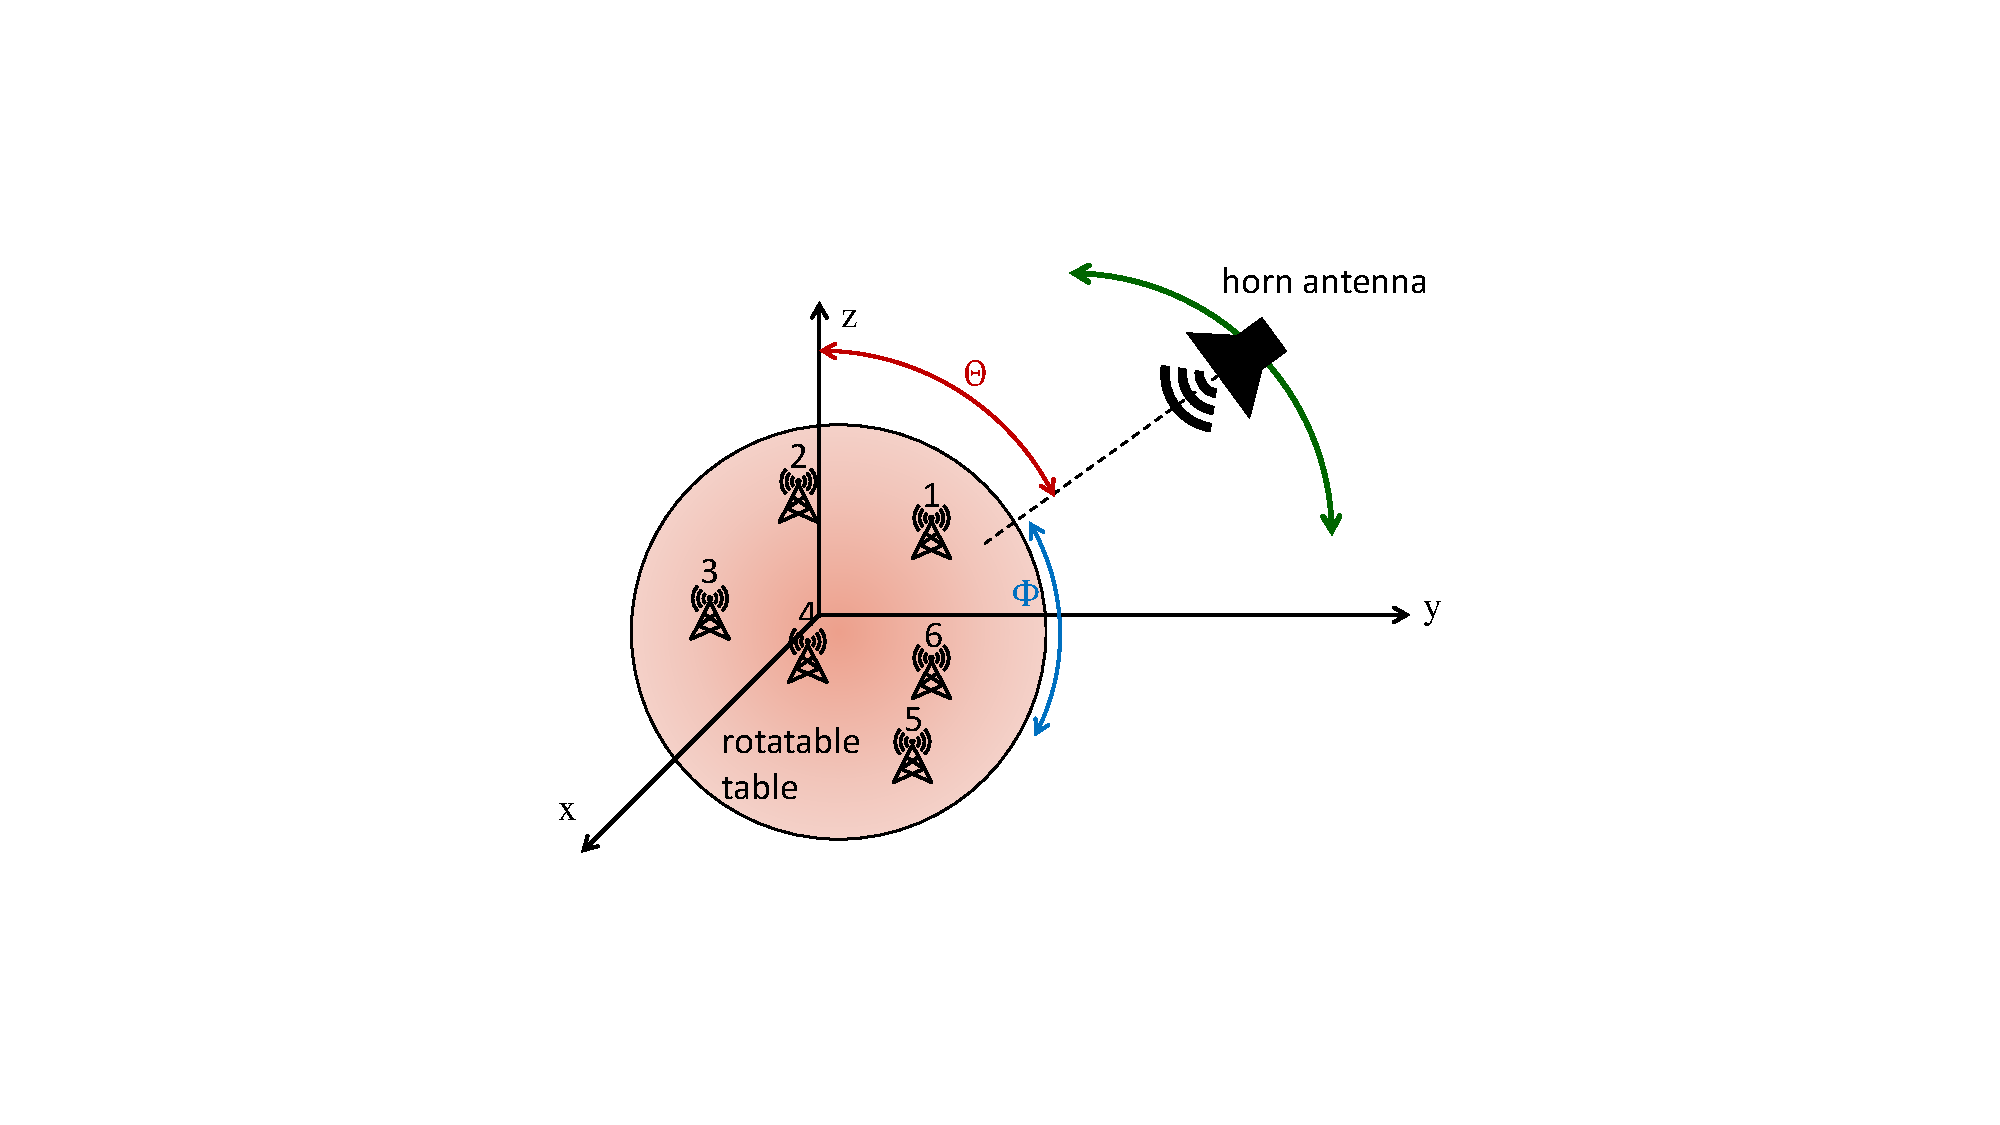
\includegraphics[trim =5cm 3cm 5cm 3cm, clip, width=0.80\textwidth]{graphics/Calibration_scenario.pdf}
	\caption{Calibration of an antenna constellation inside an antenna chamber}
	\label{fig:Calibration_scenario}
\end{figure}

In order to get information about an antenna constellation one usually calibrates the antennas using a reference antenna inside an antenna chamber. Figure \ref{fig:Calibration_scenario} depicts such a calibration figurative. After the measurement an antenna table is obtained. For the example from figure \ref{fig:Calibration_scenario} it could look like:\\
Amplitude Ratio:\\
$\vec{a}(\Theta,\,\Phi)=\mat{1\\\frac{x_2}{x_1}\\\frac{x_3}{x_1}\\\shdots\\\frac{x_6}{x_1}}$

\begin{itemize}
\item get a table of the steering vectors with different $\Theta's$ and $\Phi's$
\item between the values is interpolated (linear, quadratic, spline ...)
\end{itemize}

\subsubsection{ULA with rotation}
\begin{figure}[H]
	\centering
		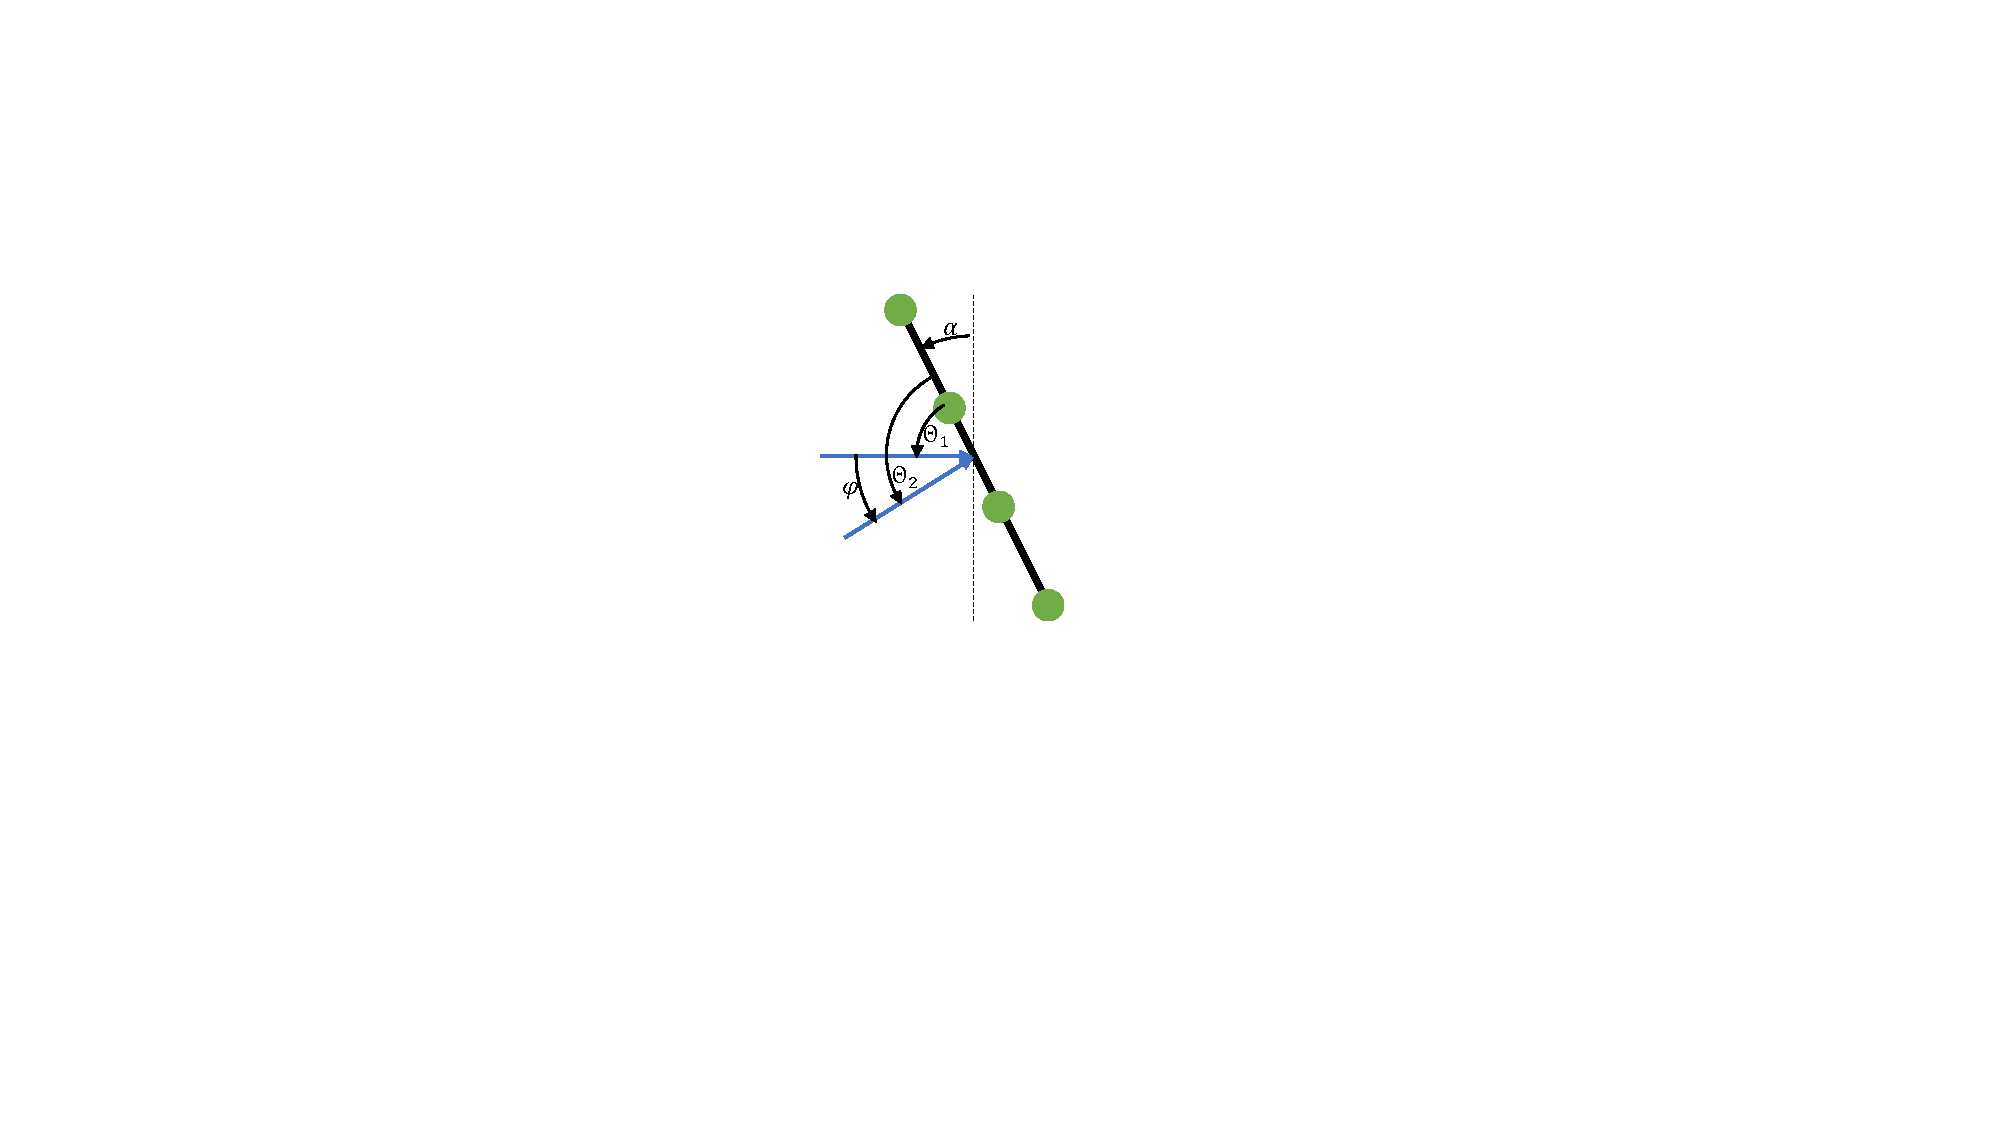
\includegraphics[trim =14cm 8cm 15.5cm 4.7cm, clip, width=0.30\textwidth]{graphics/ULA_angle.pdf}
	\caption{ULA with a rotation angle}
	\label{fig:ULA_angle}
\end{figure}

Incoming signal with two wave fronts:\\
$\vec{x}[n]=\vec{a}(\Theta_1)s_1[n]+\vec{a}(\Theta_2)s_2[n]+\vec{\nu}[n]=\underbrace{\mat{\vec{a}(\Theta_1) &\vec{a}(\Theta_2)}}_{\ma{A}}
\underbrace{\mat{s_1[n]\\s_1[n]}}_{\vec{s}}+\vec{\nu}[n]=\ma{A}\vec{s}+\vec{\nu}[n]$\\
\with $\Theta_1=\frac{\pi}{2}-\alpha$; \qquad $\Theta_2=\Theta_1+\varphi=\frac{\pi}{2}-\alpha+\varphi$ \\

Least Square: $\ma{W}^H=\ma{A}^+$\\
$\vec{\hat{s}}=\ma{A}^+\vec{x}[n]=\ma{A}^+\ma{A}\vec{s}[n]+\ma{A}^+\vec{\nu}$\\
Because $\vec{a}(\Theta_1) ,\vec{a}(\Theta_2)$ ale LID: $\ma{A}^+\ma{A}=\ma{I}$\\
\pfeil $\vec{\hat{s}}=\vec{s}[n]+\underbrace{\ma{A}^+\vec{\nu}}_{\vec{\nu'}}$\\
Observation Noise: $\vec{\nu}$ \pfeil $E[\vec{\nu}\vec{\nu}^H]=\sigma_\nu^2\ma{I}$\\
Estimation Noise: $\vec{\nu}'$\pfeil $E[\abs{\abs{\vec{\nu}}}_2^2]=\sigma_\nu^2\tr\left(\left(\ma{A}^H\ma{A}\right)^{-1}\right)$\\

Signal to Noise Ratio:\\
$SNR=\frac{E[\abs{\abs{\vec{s}}}_2^2]}{\sigma_\nu^2\tr\left(\left(\ma{A}^H\ma{A}\right)^{-1}\right)}$\\

\ \\
Example with 2 antennas and 2 wave fronts:\\
$\ma{A}=\mat{1&1\\e^{-j\pi\cos\Theta_1}&e^{-j\pi\cos\Theta_1}}=
\mat{1&1\\e^{-j\pi\sin\alpha}&e^{-j\pi\sin(\alpha-\varphi)}}$\\
$SNR=\frac{E[\abs{\abs{\vec{s}}}_2^2]}{2\sigma_\nu^2}\cdot\left( 1 -
\underbrace{ \cos\left( \pi \sin \left( \alpha-\varphi\right) -\sin\alpha \right)}_{-1 ... 1} \right)\leq \frac{E[\abs{\abs{\vec{s}}}_2^2]}{\sigma_\nu^2}$\\

Find optimal tilde angle $\alpha$ for the ULA:\\
$\alpha_{opt}=\textrm{arg}\max\limits_{\alpha}SNR = \frac{\varphi}{2}$\\
Best Result: Symmetric situation: \quad $\Theta_1=\frac{\pi}{2}-\frac{\varphi}{2}\qquad\Theta_1=\frac{\pi}{2}+\frac{\varphi}{2} $\\
$SNR_{opt}=\left.  SNR \right|_{\alpha=\frac{\varphi}{2}}=
\frac{E[\abs{\abs{\vec{s}}}_2^2]}{\sigma_\nu^2}\cdot\sin^2\left(\pi \sin \frac{\varphi}{2} \right)$\\

Example: $\varphi=22^\circ \pfeil SNR_{opt}=0.3183 \cdot SNR_{max}$